\documentclass[12pt]{report}
\usepackage{graphicx}
\graphicspath{{images/}}
\usepackage[a4paper, width=150mm, bottom=25mm, bindingoffset=6mm]{geometry}
\usepackage[super,sort&compress,comma]{natbib} 
\usepackage{sidecap}
\usepackage[toc,page]{appendix}
\usepackage{amsmath}
\usepackage{multirow}
\usepackage{tabularx}

\usepackage{xcolor}
\definecolor{codegreen}{rgb}{0,0.6,0}
\definecolor{codegray}{rgb}{0.5,0.5,0.5}
\definecolor{codepurple}{rgb}{0.58,0,0.82}
\definecolor{backcolour}{rgb}{0.95,0.95,0.92}

\usepackage{listings}
\lstset{
  language=python,
  basicstyle=\small,
  breaklines=true,
    backgroundcolor=\color{backcolour},   
    commentstyle=\color{codegreen},
    keywordstyle=\color{magenta},
    numberstyle=\tiny\color{codegray},
    stringstyle=\color{codepurple},
    basicstyle=\ttfamily\footnotesize,
    breakatwhitespace=false,         
    breaklines=true,                 
    captionpos=b,                    
    keepspaces=true,                 
    numbers=none,                    
    numbersep=5pt,                  
    showspaces=false,                
    showstringspaces=false,
    showtabs=false,                  
    tabsize=2
  }

\renewcommand{\tablename}{Tabla}

\usepackage[labelfont=bf]{caption}


%\usepackage{fancyhdr}
%\pagestyle{fancy}
%\fancyhead{}
%\fancyhead[RO, LE]{}
%\fancyfoot[LE,RO]{\thepage}
%\renewcommand{\chaptermark}[1]{\markboth{#1}{}}
%\fancyfoot[LO, CE]{\leftmark}
%\fancyfoot[CO, RE]{Tomás Di Napoli}

\usepackage{fancyhdr}

% Define the page style for pages before the index
\fancypagestyle{beforeIndex}{%
    \fancyhf{} % Clear headers and footers
    \fancyfoot[C]{\thepage} % Roman page numbering centered
    \renewcommand{\thepage}{\roman{\thepage}} % Use Roman numerals for page numbering
}

\renewcommand{\chaptermark}[1]{%
    \markboth{Cap. \thechapter\ #1}{}
}

% Define the page style for pages after the index
\fancypagestyle{afterIndex}{%
    \fancyhf{} % Clear headers and footers
    % Header configuration
    \fancyhead[LO, LE]{\leftmark}
    \fancyhead[RO, RE]{Tomás Di Napoli}
    % Footer configuration
    \fancyfoot[LE]{\thepage} % Page number on the right for even pages
    \fancyfoot[RO]{\thepage} % Page number on the left for odd pages
    \fancyfoot[LO]{Tésis de licenciatura: Caracterización de UCNPs} % Chapter name on the left for odd pages
    \fancyfoot[RE]{Tésis de licenciatura: Caracterización de UCNPs} % Chapter name on the right for even pages
}





\pagestyle{afterIndex} % Normal numbering with alternating headers/footers



\usepackage{hyperref}


\usepackage[utf8]{inputenc}
\usepackage[spanish,activeacute]{babel}
\usepackage{xcolor}

\newcommand{\todo}[1]{\textcolor{red}{#1}}
\newcommand{\done}[1]{\textcolor{blue}{#1}}

\title{Tesis de lic}
\author{Tomás Di Napoli}

\begin{document}

%\maketitle

\thispagestyle{empty}
\begin{center}

%\vspace*{2cm}
{
\includegraphics[width=5cm]{UBA_logo.png}\\}
\vspace*{2mm}
{\large Universidad de Buenos Aires\\}
{\large Facultad de Ciencias Exactas y Naturales\\}
{\large Departamento de Física\\}
%\vspace*{5mm}
%{ Intendente Güiraldes 2160, Buenos Aires, Argentina\\}
%\vspace*{5mm}


\vspace*{2cm}
{\huge \bf Renovación de un Espectrofluorímetro Obsoleto para la Caracterización de Nanopartículas de \textit{Upconversion}}

%\bf
% \vspace*{2.2cm}
% {\large A thesis submitted in partial fulfillment\\}
% {\large  of the requirements for the degree of \\}

\vspace*{1cm}
{\it {\large Tesis de Licenciatura en Ciencias Físicas} 
}

\vspace*{0.8cm}


\vspace*{6mm}
{\Large Tomás Di Napoli \\}
%{\large LU: 323/18\\
%{\small \tt azulmariabriganet@gmail.com}}

\vspace*{10mm}
{\large Dirección: Hernán Grecco\\}
\vspace*{5mm}
%{\large Colaboradores: Juan Cruz Berón\\}

\vspace*{5mm}
{\large Diciembre 2024\\}
\end{center}

\newpage

{\large TEMA: Renovación de un Espectrofluorímetro Obsoleto para la Caracterización de Nanopartículas de \textit{Upconversion}}\newline
%\vspace*{0.01cm}\newline

{\large ALUMNO: Tomás Di Napoli}\newline
%\vspace*{0.02cm}\newline

{\large LU: 551/18}
%\vspace*{0.02cm}\newline

{\large LUGAR DE TRABAJO: Laboratorio de Electrónica Cuántica, Departamento de Física, Instituto de Física de Buenos Aires, CONICET/UBA. }\newline
%\vspace*{0.02cm}\newline

{\large DIRECCIÓN: Hernán Grecco (IFIBA-UBA/CONICET)}\newline

%\vspace*{0.02cm}\newline
{\large FECHA DE INICIACIÓN: Agosto 2023}\newline
%\vspace*{0.02cm}\newline

{\large FECHA DE FINALIZACIÓN: Diciembre 2024}\newline
%\vspace*{0.02cm}\newline

{\large FECHA DE EXAMEN: 27/12/2024 }\newline
%\vspace*{0.02cm}\newline

{\large INFORME APROBADO POR: }

\vspace*{1.5cm}
\begin{center}
    \renewcommand{\arraystretch}{4.5} % Ajusta la altura de las filas
    \large % Tamaño de fuente más grande para el contenido de la tabla
    \begin{tabular}{|p{7cm}|p{7cm}|}
        \hline
        \multirow{2}{7cm}[4em]{ Autor/a \\ Tomás Di Napoli} & \multirow{2}{5cm}[4em]{ Jurado \\ Dr. Christian T. Schmiegelow} \\
        \hline
         \multirow{2}{7cm}[4em]{ Director/a \\ Dr. Hernán Grecco } & \multirow{2}{5cm}[4em]{ Jurado \\ Dra. María Gabriela Capeluto} \\
        \hline
        \multirow{2}{7cm}[4em]{ Profesor/a de la Tesis de Licenciatura\\Dra. Silvina Ponce Dawson} & \multirow{2}{5cm}[4em]{ Jurado\\ }\\
        \hline
    \end{tabular}
\end{center}

\pagenumbering{roman}

\chapter*{Agradecimientos}

\chapter*{Resumen}

La fotoluminiscencia es la emisión de luz de cualquier forma de materia debida a una absorción previa de fotones. 
Esta propiedad es frecuentemente utilizada en microscopía con aplicaciones bioquímicas y biológicas, generalmente a través de agentes fotoluminiscentes como tintas orgánicas, proteínas fluorescentes y puntos cuánticos semiconductores. 
La mayoría de estos agentes exhiben corrimiento de Stokes, conversión de fotones de alta energía (UV-vis) a baja energía (rojo-NIR).
En este trabajo se estudian las nanopartículas de \textit{upconversion} (UCNP), redes cristalinas dopadas con lantánidos que interactúan entre sí para absorber fotones en el NIR y re-emitirlos en el UV-VIS.

En particular, se desarrolló tanto el \textit{hardware} como el \textit{software} de una plataforma capaz de la caracterización óptica de estas nanopartículas, tomando como base un espectrofluorímetro comercial obsoleto Horiba PTI Quanta Master 400.
Se renovó el instrumento reemplazando la PC y electrónica de control por una CPU y FPGA Red Pitaya.
Se desarrollaron dos paquetes de Python, \textit{redpipy} y \textit{refurbishedPTI}, que perimten controlar los monocromadores y leer la señal del PMT del fluorímetro.
Ambos paquetes se desarrollaron de forma tal que puedan ser reutilizados: \textit{redpipy} consiste en una interfaz de aplicación del programador (API) para controlar la Red Pitaya, y \textit{refurbishedPTI}, que implementa el control del fluorímetro, no es particular de este instrumento, sino que se puede utilizar para controlar cualquier fluorímetro con monocromadores y PMT.
Para asegurarse de que el fluorímetro renovado implemente las funcionalidades correctamente se caracterizó en profundidad el sistema de detección de fotones.
Además, se expandieron las capacidades del fluorímetro original agregando un láser externo pulsado, con una fuente de potencia variable, que permite realizar mediciones de tiempo de vida aplicando la técnica \textit{Time-Correlated Single Photon Counting} (TCSPC).

Por último, se utilizó esta plataforma para caracterizar un lote de UCNP compuestas por una matriz cristalina de fluoruro de ítrio NaYF$_4$ y dopada con iones lantánidos erbio Er$^{3+}$ e iterbio Yb$^{3+}$.
Para eso, se midió el espectro de emisión estacionario al excitar de forma continua con un láser de 976 nm en un rango de densidades de potencia de excitación desde 16 mW cm$^{-1}$ hasta 80 mW cm$^-1$.
Asimismo, se midieron los tiempos de vida para los picos de emisión más intensos, y se comparó el resultado a dos potencias de excitación distintas.
Se observó un comportamiento lineal en función de la potencia para los espectros estacionarios, y no se observaron diferencias significativas entre los tiempos de vida a distintas potencias.

\textbf{Palabras clave:} \textit{upconversion}, luminiscencia, espectrofluorimetría.






\tableofcontents


\chapter{Introducción}
\pagenumbering{arabic}
En 1565, el médico y botanista Nicolás Monardes reportó el peculiar color azul que tomaba una infusión de madera mexicana usada para tratar enfermedades de riñón y urinarias. Este efecto ya era conocido por los Aztecas, que lo utilizaban para asegurarse que la valiosa madera no fuera falsificada. Monardes escribe en su libro \cite{valeur_introduction_2012}

\begin{quote}
    \textit{Asegúrate de que la madera torne el agua azulada, de lo contrario, es una falsificación. De hecho, ahora traen otro tipo de madera que torna el agua amarilla, pero no sirve; solo el tipo que torna el agua azulada es genuina.}
\end{quote}  

\noindent Años más tarde, en 1845, el matemático Sir John Herschel describió el efecto similar que producía una solución transparente de quinina, una sustancia presente en el agua tónica, que reflejaba \flqq un color azul celestial hermoso y extremadamente vívido\frqq.
Herschel usó un prisma para comprobar que la dispersión causada por la quinina sólo se observaba al iluminar la solución con la parte azul del espectro.
El mismo análisis para la luz emitida reveló luz azul, verde, y una pequeña cantidad de amarillo.
En esa misma época, el físico Sir George Gabriel Stokes publicó \textit{On the Refrangibility of Light}, un trabajo explicando experimentos con múltiples sustancias que exhibían este tipo de comportamientos, entre ellas incluida la quinina.
Uno de sus experimentos más importantes consistía en formar el espectro solar a partir de un prisma, para luego mover un tubo de ensayo con la solución de quinina a través de sus colores.
La solución permanecía transparente al ser iluminada por la parte visible del espectro, pero al llegar a la zona ultravioleta (invisible al ojo humano), la muestra se iluminó con luz azul brillante.
Además de concluir que la luz siempre se dispersaba con longitudes de onda mayores a las de incidencia, afirmación que luego se conocería como corrimiento de Stokes, llamó a este fenómeno \textit{fluorescencia} \cite{valeur_introduction_2012}.

En 1888, el físico Eilhardt Wiedmann introdujo el término luminiscencia para referirse a los fenómenos lumínicos que no están determinados por un aumento en la temperatura de los materiales.
Entre ellos están la fosforescencia y la fluorescencia.
Actualmente ambos tienen aplicaciones en múltiples áreas distintas del conocimiento y la tecnología. 
Es particularmente destacable su éxito como herramienta para estudiar la estructura y dinámica de la materia viva, gracias la sensibilidad al micro-entorno de las moléculas fluorescentes, lo que resulta en una alta resolución espacial y temporal. 
Por ejemplo, la microscopía de fluorescencia consiste en iluminar la muestra con una longitud de onda y detectar su fluorescencia en otra, permitiendo filtrar el fondo de la imagen \cite{valeur_introduction_2012}.
Técnicas dinámicas como la microscopía de imágenes de tiempo de vida de fluorescencia (FLIM) o fosforescencia (PLIM) dan lugar a conocer el entorno químico en el que se encuentran distintas proteinas, como su PH, viscosidad, temperatura, entre otras cantidades \cite{suhling_fluorescence_2015} \cite{baggaley_timeresolved_2015}.
Si bien en el siglo 19 ya se sabía que los mecanismos de emisión de luz de estos fenómenos no estaban vinculados al aumento de temperatura de los materiales, no fue hasta el desarrollo de la mecánica cuántica a principos del 20 que se entendió su causa: la luminiscencia está dada por la transición entre distintos estados de energía de los electrones.

\section{Luminiscencia}


\begin{figure}
    \centering
    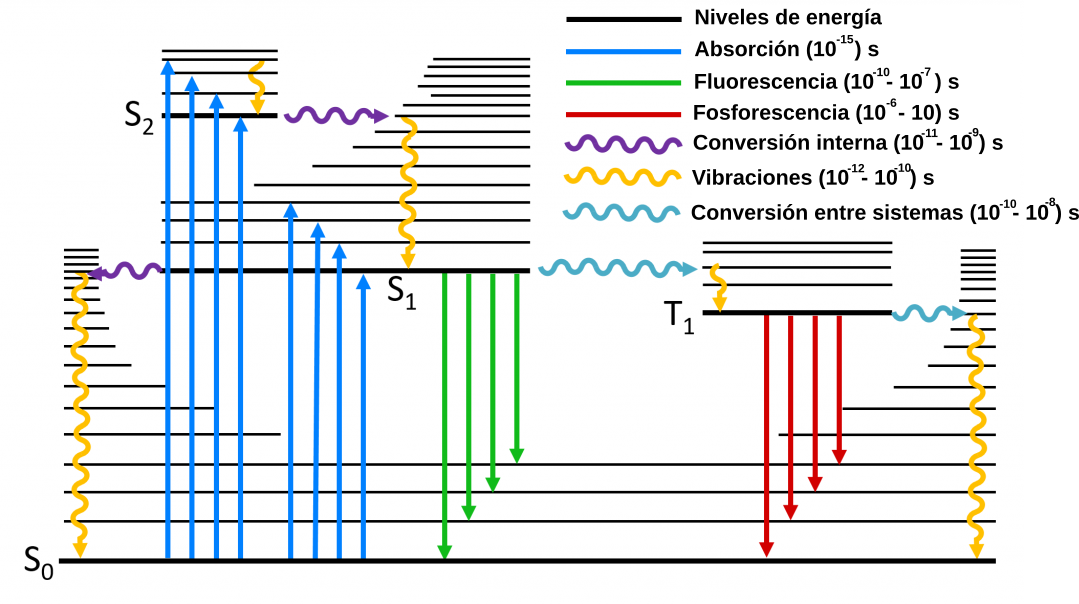
\includegraphics[width=\textwidth]{jablonski}
    \caption{\textbf{Diagrama de Jablonski.} En negro se ven los niveles de energía, crecientes en el eje vertical. Las flechas de colores muestran las transiciones posibles.}
    \label{fig:jablonski}
\end{figure}

\subsection{Espectroscopía estática}

La luminiscencia es la emisión de fotones mediante la transición de un electron en un estado excitado con energía $E_e$ a otro con energía $E_k < E_e$.
Este proceso suele ilustrarse a través de un diagrama de Jablonski (\textbf{Fig. \ref{fig:jablonski}})\footnote{Tomado de \href{https://edinst.com/wp-content/uploads/2019/02/JablonskiDiagramFull-1024x604.png}{https://edinst.com/wp-content/uploads/2019/02/JablonskiDiagramFull-1024x604.png}}.
En un diagama de Jablonski se muestran los niveles de energía electrónicos del material luminiscente junto con las posibles transiciones entre ellos.
En el diagrama se ven los estados singlete $S_0$, $S_1$ y $S_2$, y el estado triplete $T_1$.
Todo proceso luminiscente comienza con la absorción de un fotón, lo que lleva al electrón a un estado más energético.
Estas absorciones ocurren en un lapso de $10^{-15}$ s, un tiempo suficientemente corto como para que los desplazamientos de los núcleos del sistema sean despreciables \cite{lakowicz_principles_2006}.
La diferencia de energía entre estos estados es típicamente del orden de los eV.
A su vez, un electrón en un dado estado electrónico puede estar en distintos estados vibracionales, aunque estos estados están separados por energías del orden de las décimas de eV.
Las transiciones entre estados vibracionales también son posibles y ocurren en un lapso de $10^{-12}$ a $10^{-10}$ segundos.

La sucesión de este tipo de transiciones da lugar a la fluorescencia: un electrón absobe un fotón altamente energético, excitándolo a un estado electrónico de mayor energía con vibraciones.
Rápidamente sus oscilaciones se relajan, dejándolo en un estado electrónico excitado, pero con baja energía vibracional.
Por último, el electrón vuelve a su estado fundamental re-emitiendo un fotón, pero esta vez de menor energía que el que había absorbido.
La fluorescencia tiene tiempos típicos de $10^{-10}$ a $10^{-7}$ segundos.
El método más usual para caracterizar un material fluorescente, o luminiscente en general, es a través de su espectro de emisión y de absorción.
Alternativamente, uno puede medir el espectro de excitación, que está fuertemente relacionado con el de absorción.
El proceso para medir cada uno es:

\begin{itemize}
    \item \textbf{Emisión:} consiste en medir la intensidad de luz emitida por la muestra en un rango amplio de longitudes de onda $\Delta \lambda_{em}$, al ser excitada por una longitud de onda fija $\lambda_{ex}$.
    \item \textbf{Absorción:} requiere medir la intensidad de luz que absorbe la muestra. Esto generalmente se logra excitando una solución de la sustancia en un rango de longitudes de onda y midiendo la cantidad de luz transmitida en cada caso.
    \item \textbf{Excitación:} para obtener este espectro se debe medir la intensidad de luz emitida por la muestra una dada longitud de onda $\lambda_{em}$, y barrer la excitación en un rango $\Delta \lambda_{ex}$.
\end{itemize}

\noindent La figura (\textbf{\ref{fig:fluoresceina}}) muestra el espectro de absorción y de emisión de la fluoresceina, una tinta orgánica utilizada en distintas técnicas de diagnóstico médico \cite{fluoresceina_1,fluoresceina_2}.
Los espectros dejan en evidencia la fluorescencia de la molécula: absorbe fotones de $457$ y $486$ nm, es decir $2.71$ eV y $2.55$ eV respectivamente, y emite con mayor intensidad en $523$ nm, equivalente a $2.37$ eV.
Previsiblemente, la diferencia de energía es de $\sim 0.2$ eV, en el rango de energías vibracionales.


\begin{SCfigure}
    \centering
    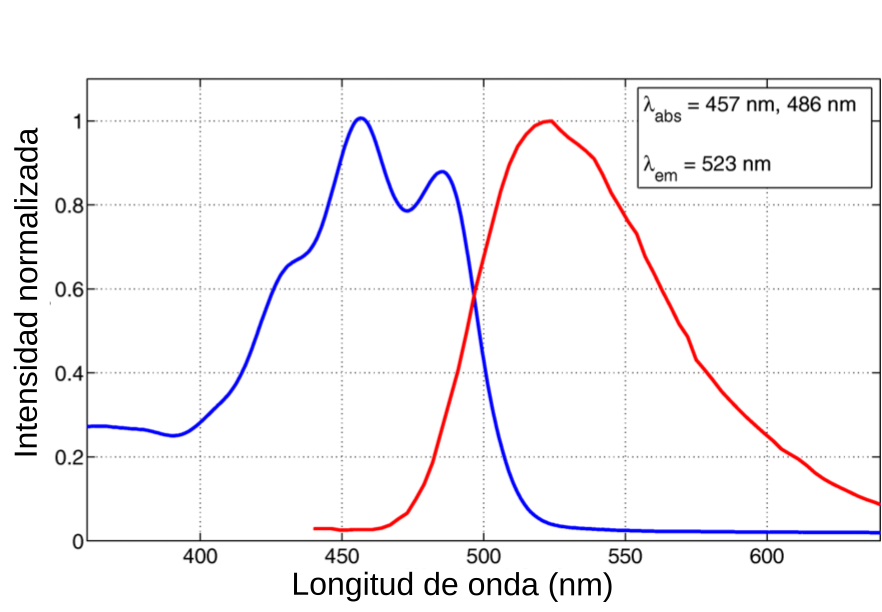
\includegraphics[width=0.7\textwidth]{fluoresceina_espectro.png}
    \caption{\textbf{Espectro de la Fluoresceina} diluida en etanol, tanto de absorción (azul) como de emisión (rojo). El cuadro muestra los picos de absorción en $\lambda_{abs}=457$ nm y 486 nm, y de emisión en $\lambda_{em}$ = 523 nm. Tomada y adaptada de \cite{kristoffersen_testing_2018}.}
    \label{fig:fluoresceina}
\end{SCfigure}

Otro tipo de mecanismos presentes en los materiaes luminiscentes son la conversión interna y la conversión entre sistemas.
Ambos consisten en transiciones entre estados electrónicos excitados, el primero es entre estados de la misma multiplicidad, en general singlete-singlete, y el segundo se da entre estados singlete-triplete \cite{valeur_characteristics_2012}.
La conversión entre sistemas, que ocurre en el orden de $10^{-10}$ a $10^{-9}$ segundos, es la responsable de la fosforescencia.
La fosforescencia es la transición de un electrón en un estado excitado triplete a un estado singlete de menor energía.
A diferencia de las transiciones fluorescentes, las transiciones triplete-singlete están prohibidas por las reglas de selección de la mecánica cuántica \cite{demtroder_emission_2010}.
Por este motivo, los tiempos característicos de la fosforescencia son mucho mayores, del orden de $10^{-6}$ hasta $10$ segundos.
Además de los espectros de absorción, emisión y excitación, los tiempos de estas transiciones son de gran relevancia para caracterizar a los materiales luminiscentes.

\subsection{Espectroscopía dinámica} \label{sec:dinamica}



Se le llama tiempo de vida medio al tiempo promedio que el electrón pasa en un estado excitado de energía.
La caracterización del tiempo de vida medio no solo brinda información del elemento luminiscente, sino también de su entorno.
Es necesario hablar de tiempos medios porque las transiciones son un fenómeno fundamentalmente cuántico, y por lo tanto un proceso aleatorio.
Además, la mayoría de mediciones de luminiscencia se hacen con una muestra que presenta grandes cantidades de los elementos ópticamente activos, por lo que también hay un efecto aleatorio propio de esa estadística.

\begin{SCfigure}
    \centering
    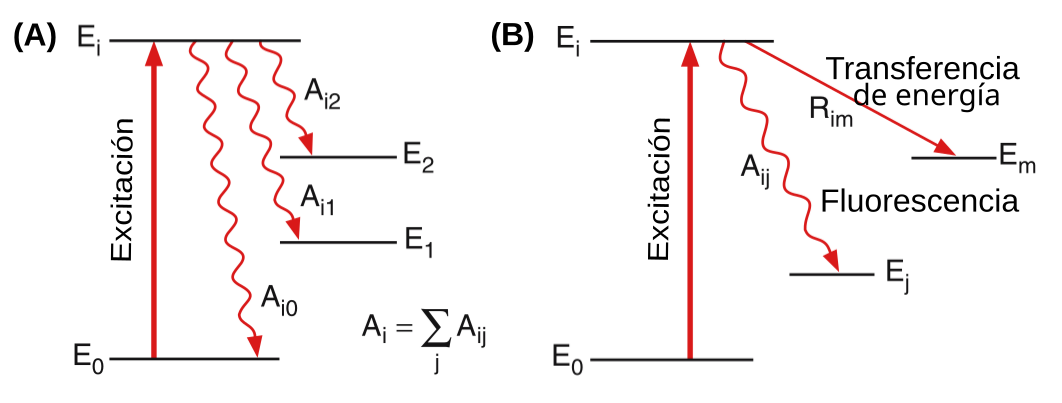
\includegraphics[width=0.7\textwidth]{transiciones_tiempo.png}
    \caption{\textbf{Diagrama de Jablonski} con transiciones que contribuyen al tiempo de vida.\textbf{(A)} Sólo transiciones de fluorescencia. \textbf{(B)} Transiciones de fluorescencia y choques. Tomado y adaptado de \cite{demtroder_emission_2010}.}
    \label{fig:transiciones_tiempo}
\end{SCfigure}

Si se tienen $N_i$ átomos en un estado excitado con energía $E_i$ y se asume que la probabilidad de transición a un estado de menor energía $E_j$ es constante en el tiempo se obtiene que

\begin{equation} \label{eq:lifetime}
    \frac{dN_i}{dt} = A_{ij} N_i \implies N_i(t) = N_i(0)e^{A_i t},
\end{equation}

\noindent donde $A_{ij}$ es una constante llamada coeficiente de Einstein, y $A_i = \sum_{j} A_{ij}$ tiene en cuenta la probabilidad del electrón decaiga a cualquier estado con $E_j < E_i$ (ver \textbf{Fig. \ref{fig:transiciones_tiempo}A}) \cite{demtroder_emission_2010}.
Como sabemos que un electrón emite un fotón al desexcitarse, la ecuación (\ref{eq:lifetime}) nos dice que al dejar de iluminar una muestra esperamos que se emitan fotones exponencialmente distribuidos en el tiempo.
Es decir que si tenemos un detector de fotones, medimos con precisión el tiempo en el que dejamos de iluminar, y hacemos un histograma de los tiempos en los que detectamos un fotón, las alturas de sus barras deberían seguir una exponencial.
Además sabemos que la relación entre el tiempo de vida y el parámetro de la exponencial es $\tau_i = 1/A_i$, por lo que es posible ajustar una exponencial a la altura de las barras para medirlo.
Exactamente eso es lo que se hace en \textit{Time-Correlated Single Photon Counting} (TCSPC, ver sección \ref{sec:intro_tcspc}), una de las técnicas más comunes para medir tiempos de vida.

La ecuación (\ref{eq:lifetime}) sólo tiene en cuenta las transiciones fluorescentes del átomo, pero como explicamos en la sección anterior, éstas no son las únicas.
Además, generalmente los átomos están en entornos que inducen transiciones no radiativas, como transferencia de energía a otros átomos, o colisiones con átomos vecinos (\textbf{Fig. \ref{fig:transiciones_tiempo}B}). 
Suponiendo que se induce una nueva probabilidad de desexcitación no radiativa $R_i$ por transferencia de energía, y siguiendo la lógica anterior, la tasa de cambio de cantidad de átomos $N_i$ en el estado $i$ es

\begin{equation} \label{eq:lifetime_choques}
    \frac{dN_i}{dt} = (A_{ij} + R_i) N_i \implies N_i(t) = N_i(0)e^{(A_i + R_i) t},
\end{equation}

\noindent y por lo tanto su tiempo de vida efectivo $\tau_{eff} = 1/(A_i + R_i)$. 
La implicancia de este fenómeno es muy fuerte: es posible obtener información del entorno microscópico de un material luminiscente al medir su tiempo de vida \cite{ryder_timedomain_2001}.

Para poder aprovechar estas propiedades de los materiales luminiscentes es necesario poder medir precisamente tanto sus espectros estacionarios como los dinámicos. 
En la próxima sección comentamos brevemente cuáles son los instrumentos y técnicas que se implementan más comunmente para hacer este tipo de mediciones.


\section{Instrumentación para espectrometría de fluorescencia}

\subsection{El espectrofluorímetro}

Para caracterizar la respuesta óptica de una sustancia, generalmente se desea registrar tanto el espectro de excitación como el de emisión. 
El instrumento científico por excelencia para realizar estas mediciones es el espectrofluorímetro. 
Fundamentalmente, este instrumento permite realizar mediciones de la intensidad de luz que emite una muestra, haciendo escaneos en longitud de onda de emisión y excitación.
Adicionalmente, algunos pueden realizar mediciones de tiempo de vida resueltas, escaneos sincrónicos con alguna señal y mediciones de anisotropía en la polarización de materiales luminiscentes.
Estas capacidades son fundamentales para investigaciones en diversas disciplinas científicas, incluyendo química, bioquímica, farmacología, ciencias ambientales, ciencia de materiales y biomedicina.
El objetivo principal de un espectrofluorímetro es obtener los espectros de emisión y de excitación de una muestra.
Para lograr este objetivo, el instrumento debe ser capaz de iluminar la muestra con múltiples longitudes de onda diferentes y registrar su respuesta a cada una de ellas.

La Figura 2.1 muestra un diagrama esquemático de un espectrofluorímetro genérico.
Este instrumento incluye todos los componentes fundamentales para cumplir su función. 
Utiliza una lámpara de espectro amplio que funciona como fuente de luz de alta intensidad para un rango extenso de longitudes de onda. 
Posteriormente la luz es filtrada por un monocromador de excitación que permite seleccionar la longitud de onda con la que se desea iluminar a la muestra.
La luz de excitación seleccionada se enfoca sobre la muestra colocada en la cámara principal, cuya luminiscencia, generalmente con una longitud de onda mayor que la luz de excitación, es filtrada por el monocromador de emisión.
Los monocromadores suelen estar motorizados, lo que permite que el escaneo sea automático. 
La luz restante llega a un detector, usualmente un tubo fotomultiplicador (PMT), un detector muy sensible que convierte fotones en corriente eléctrica.
El espectrofluorímetro emplea diversas técnicas para reducir la luz parásita (longitudes de onda diferentes a la deseada), como el diseño en ángulo de 90° entre los brazos de excitación y emisión, y un compartimento hermético pintado de negro no reflectante.
La señal del PMT es procesada electrónicamente, digitalizada y analizada en una computadora. 
Este sistema también controla los monocromadores y la adquisición de datos, además de permitir al usuario ajustar parámetros y facilitar la visualización y análisis.
A menudo, se incorporan componentes adicionales en el camino óptico, como obturadores, polarizadores, divisores de haz y otros elementos ópticos, para estudiar diferentes propiedades de la muestra.

\begin{SCfigure}
     \centering
     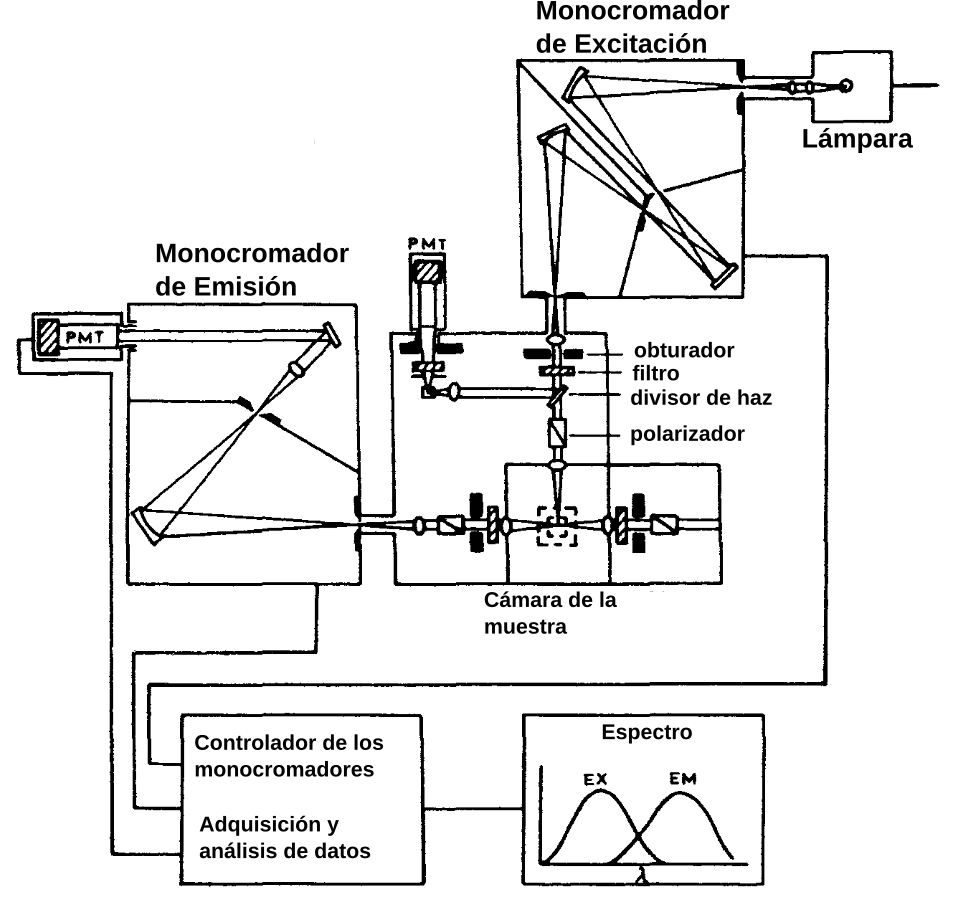
\includegraphics[width=0.6\textwidth]{spectrometer_diagram_lako_modif.png}
     \caption{
    \textbf{Diagrama de un espectrofluorímetro genérico.}
    La luz traza un camino que comienza en la lámpara (zona superior derecha) y termina en el PMT de detección (centro-izquierda). Después de salir de la lámpara, la luz es filtrada por un monocromador y luego enfocada sobre la muestra. La luz reemitida pasa por otro monocromador y termina en el PMT. La señal se lee con un sistema de control que la digitaliza y para luego ser procesada por una PC que construye los espectros. Figura tomada y adaptada de \cite{lakowicz_principles_2006}.
    }
     \label{fig:spec_diagram_lako}
\end{SCfigure}


\todo{El mio es el más comun, pero no es el único que existe}

\subsection{Epectrofluirimetros en argentina y obsolescencia}

Actualmente, el Departamento de Física de la FCEyN-UBA no cuenta con espectrofluorímetros para la caracterización de espectros de excitación y emisión.  
Para realizar este tipo de mediciones, la facultad dispone del laboratorio de fotoquímica del Instituto de Química Física de los Materiales, Medio Ambiente y Energía (INQUIMAE), que cuenta con tres espectrofluorímetros con distintas características, pero que tienen algo en común: ningún equipo tiene menos de 20 años, el más antigüo llegando a los 40 años de uso.
La disparidad en la antigüedad y funcionalidad de los instrumentos es un fenómeno común en laboratorios de investigación en países como Argentina, donde la inversión en ciencia es escasa o poco regular en el tiempo \cite{cioccaRealityScientificResearch2017}. 
Ante esta realidad, los institutos suelen priorizar la adquisición de equipos con nuevas capacidades, en lugar de renovar instrumentos existentes por versiones más modernas.  
Esto es posible gracias a la precisión y robustez de las partes mecánicas de los instrumentos, pero la obsolescencia de los equipos antiguos plantea problemas a largo plazo, especialmente cuando sus plataformas de control quedan desactualizadas.  
Con el tiempo, se vuelve complicado operar estos instrumentos, ya que los mecanismos de extracción de datos, como los disquetes, dejan de estar disponibles en el mercado. 
Aún más crítico es que el funcionamiento del equipo depende de la computadora de control, la cual utiliza placas y puertos que ya no se fabrican ni se consiguen en el mercado actual.  
El problema de la obsolescencia en instrumentos científicos afecta desproporcionadamente a instituciones con bajo presupuesto, ampliando la brecha de accesso a instrumentos de investigación avanzados.

Esto ha llevado a un auge en el desarrollo de instrumentos científicos accesibles y de bajo costo \cite{wenzel_open_2023, arancio_inequalities_2023}, particularmente en áreas como instrumentación, microscopía, espectroscopía y adquisición de datos \cite{jameson_fluorescent_1989, li_optical_2022, hu_fluorescent_2022}.
Las iniciativas de hardware abierto hacen que los diseños y la documentación estén disponibles de forma gratuita para que cualquier persona pueda usarlos, construirlos y modificarlos \cite{powell_democratizing_2012, oellermann_open_2022}.
Por ejemplo, la plataforma Arduino ha proporcionado una plataforma de desarrollo de electrónica económica y fácil de usar basada en un microcontrolador (https://www.arduino.cc/).
El OpenFlexure Microscope es un microscopio de código abierto que cuesta menos de 100 USD construir \cite{collins_robotic_2020}.
Asimismo, recientemente se desarrolló un espectrómetro basado en Raspberry Pi que cuesta menos de 400 EUR \cite{tunens_optical_2024}.
El software y los lenguajes de código abierto, como Python (http://www.python.org), que cuentan con bibliotecas numéricas y de instrumentación como NumPy \cite{harris_array_2020} y PyVISA \cite{grecco_pyvisa_2023}, han desempeñado un papel clave al reducir las barreras de entrada y facilitar la creación rápida de prototipos.
Cabe destacar que han surgido empresas enfocadas en hardware parcialmente o completamente abierto. Por ejemplo, OpenBCI (https://openbci.com/), que ofrece sistemas EEG de bajo costo para interfaces cerebro-computadora, y Opentrons (https://opentrons.com/), que proporciona soluciones de manejo de líquidos para la automatización de laboratorios.


\subsection{Medición de tiempos de vida: \textit{Time-Correlated Single Photon Counting}} \label{sec:intro_tcspc}


\begin{figure}
    \centering
    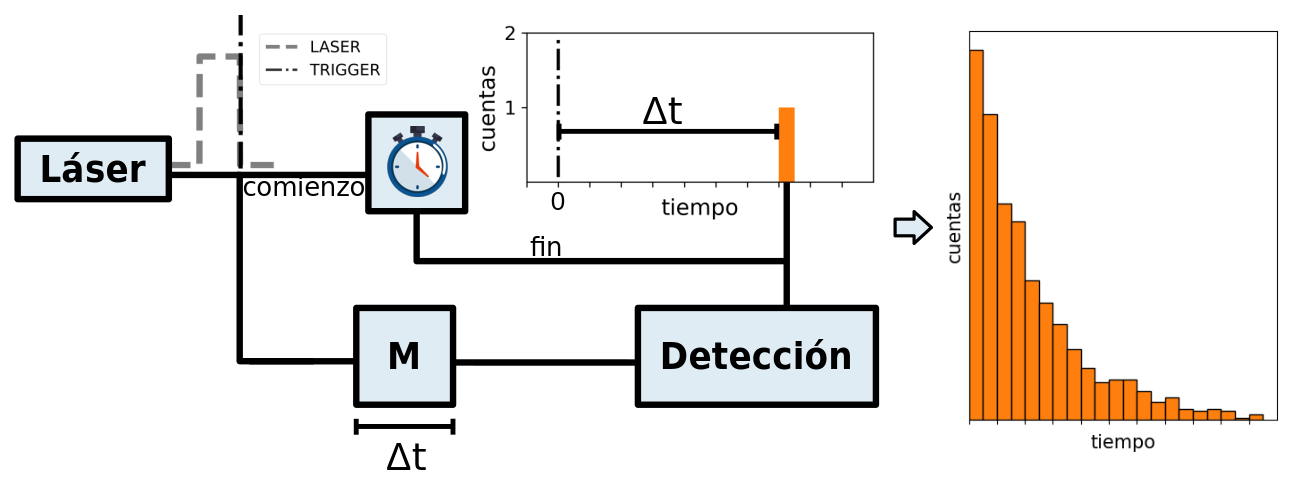
\includegraphics[width=\textwidth]{tcspc.png}
    \caption{\textbf{Diagrama de TCSPC.} El láser envía un pulso que excita a la muestra e inicia un cronómetro. La muestra tarda un tiempo $\Delta t$ en re-emitir. El sistema de detección detecta la luz y pone detiene el cronómetro. Se registra el tiempo $\Delta t$. Al repetir el experimento múltiples veces se crea el histograma de cuentas en función del tiempo (derecha). Adaptada de \cite{bujjamer2020}.}
    \label{fig:tcspc}
\end{figure}

Muchos espectrofluorímetros comerciales tienen la capacidad de medir tiempos de vida del orden de los nanosegundos. 
Sin embargo, existen materiales luminiscentes, como los fosforescentes, presentan tiempos de vida del orden de los cientos de microsegundos en adelante.
Aunque esto alivia la necesidad de una electrónica rápida y costosa, contradictoriamente hace que no se pueda medir su tiempo de vida en instrumentos comerciales, ya que los valores típicos están muy alejados del rango en el que operan \cite{bujjamer2020}.

Existen distintas técnicas para medir el tiempo de vida \cite{becker_fluorescence_2012}, pero la más implementada es \textit{Time-Correlated Single Photon Counting} (TCSPC).
TCSPC es una técnica digital que cuenta fotones correlacionados temporalmente con respecto a un pulso de excitación.
Un diagrama de esta técnica de medición se puede ver en la figura (\textbf{\ref{fig:tcspc}}).
El experimento comienza con un pulso de excitación, que tiene dos tareas: (i) excitar a la muestra y (ii) iniciar algún tipo de cronómetro.
La muestra se excita repetidamente utilizando una fuente de luz pulsada, comunmente un láser.
Cada pulso es monitreado, produciendo una señal de inicio que activa el contador del cronómetro.
Usualmente, para esta tarea se usa un conversor de tiempo a amplitud (TAC).
La luz re-emitida por la muestra llega al sistema de detección, que además de detectar el pulso es el responsable de detener el cronómetro.
Al final de esta medición se obtiene el tiempo que tardó el fotón en llegar al detector.
Al repetir este exprimento múltiples veces, se construye un histograma de cuentas de fotones en función del tiempo.
De acuerdo a lo explicado en la sección \ref{sec:dinamica}, para el caso en que sólo hay transiciones de fluorescencia, las alturas de las barras de este histograma deberían seguir una distribución exponencial con tiempo característico $\tau$, el tiempo de vida.

Además de los sistemas fluorescentes y fosforescentes existen otros sistemas en los que distintos centros ópticamente activos interactúan entre sí de forma no lineal, resultando en que la solución a la ecuación equivalente a \ref{eq:lifetime_choques} no sea una exponencial decreciente.
En la próxima sección introduciremos a las nanopartículas de \textit{upconversion}, un sistema con estas propiedades.


\section{Nanopartículas de \textit{upconversion}} \label{sec:intro_ucnp}

\subsection{Luminiscencia de las UCNP}

Las nanopartículas de \textit{upconversion} (UCNP) consisten en una matriz cristalina con dimensiones nanométricas dopada con iones lantánidos trivalentes.
El término \textit{upconversion}, que traducido literalmente del inglés sería conversión ascendente, surge la capacidad de las UCNP de absorber fotones de baja energía, generalmente en el infrarrojo cercano (NIR) y re-emitirlos en el espectro visible y ultravioleta (UV-VIS).
Esta propiedad es útil en múltiples áreas distintas.
Por ejemplo, se pueden utilizar como trazadores ópticos en microscopía para etiquetar células, manipular drogas a nivel microscópico y en teranósticos, una técnica de diagnóstico usada comunmente en tratamientos de medicina nuclear \cite{shen_lanthanidedoped_2013,guryev_ucnpbased_2020,haase_upconverting_2011}.
Al absorber en el infrarrojo presentan una ventaja ante otros fluoróforos, ya que en este rango de longitudes de onda la luz es menos dispersada por los tejidos, además de causar menos daño biológico.
Esta capacidad de convertir luz en el NIR al UV-VIS también se puede aprovechar para mejorar la eficiencia de celdas solares, que no son capaces de convertir fotones en el NIR a energía eléctrica \cite{hao_enhancing_2017}.
Otras potenciales aplicaciones de las nanopartículas incluyen su uso para el diseño de pantallas transparentes, termómetros nanométricos y detectores de moléculas fluorescentes en agua \cite{hong_orthogonal_2021,savchuk_thermochromic_2016, bujjamer_first_2021}.

El motivo de la conversión ascendente de las nanopartículas está dado por la interacción entre los iones lantánidos con las que son dopadas.
Los lantánidos son los elementos del sexto período de la tabla periódica, y se caracterizan por ser los elementos que completan los niveles electrónicos $4f$, comenzando con el lantano y finalizando con el lutecio.
Aunque esos son sus niveles más energéticos sin completar, los niveles $5s^25p^6$ corresponden a funciones de onda más externas que las $4f$, generando una especie de capa protectora para los electrones de valencia \cite{lanthanides}.
La consecuencia de esto son bandas muy angostas en sus espectros de emisión, ya que sus propiedades se ven poco afectadas por los factores externos. 
Por este motivo, los niveles de energía de los iones lantánidos dentro de la matriz cristalina son similares sus niveles cuando están libres\cite{nadort_lanthanide_2016}.
La luminiscencia de estos iones se da por las transiciones entre los niveles $f-f$ con la misma paridad.
Si bien las reglas de selección de la mecánica cuántica establecen que estas transiciones están prohibidas por dipolo eléctrico, para los lantánidos que se encuentran en las UCNP estas condiciones se ven relajadas por la asimetría de la red cristalina y la interacción entre ellos \cite{basics_of_lanthanide}.
Estas transiciones semi-prohibidas de los lantánidos se ven reflejadas en los largos tiempos de vida de sus estados excitados, que suelen ser del orden de los cientos de microsegundos hasta los milisegundos.

En el desarrollo de esta tésis utilizamos UCNPs formadas por una matriz cristalina de fluoruro de ítrio NaYF$_4$ dopadas con iones lantánidos de erbio Er$^{3+}$ e iterbio Yb$^{3+}$ (\textbf{Fig. \ref{fig:ucnp_niveles}B}).
Las nanopartículas cuentan con una capa externa de matriz sin dopaje que aumenta fuertemente su eficiencia (ver \textbf{Fig. \ref{fig:ucnp_niveles}A})\cite{mai_highly_2007,caracterizacion_ucnps_unicas}.
La figura (\textbf{\ref{fig:ucnp_niveles}C}) muestra el diagrama de niveles del Yb y el Er, y la (\textbf{\ref{fig:ucnp_niveles}D}) los mecanismos más comunes de interacción entre ellos.

El sistema Yb-Er forma un sistema sensibilizador-activador, donde el sensibilizador, en este caso el iterbio, tiene una gran sección eficaz por lo que tiene una alta probabilidad de absorber fotones.
El Yb en particular tiene su pico de absorción en $\sim 980$ nm, lo que excita a su electrón de valencia al nivel $^2$F$_{5/2}$.
Por otro lado el Er, el activador del sistema, también tiene una banda de absorción centrada en 980 nm que excita la transición $^4$I$_{15/2} \rightarrow ^4$I$_{11/2}$.
A su vez, presenta sucesivos niveles de energía mayores al $^4$I$_{11/2}$ equiespaciados con una energía de 980 nm.
La combinación entre este esquema de niveles tipo escalera y los largos tiempos de vida de los lantánidos dan el origen a la conversión ascendente: los electrones del Er logran excitarse múltiples veces antes de decaer a su estado fundamental.
Esto hace que la transición final sea de mayor energía que los fotones con los que se iluminó a la muestra, re-emitiendo en el espectro UV-VIS.

\begin{figure}
    \centering
    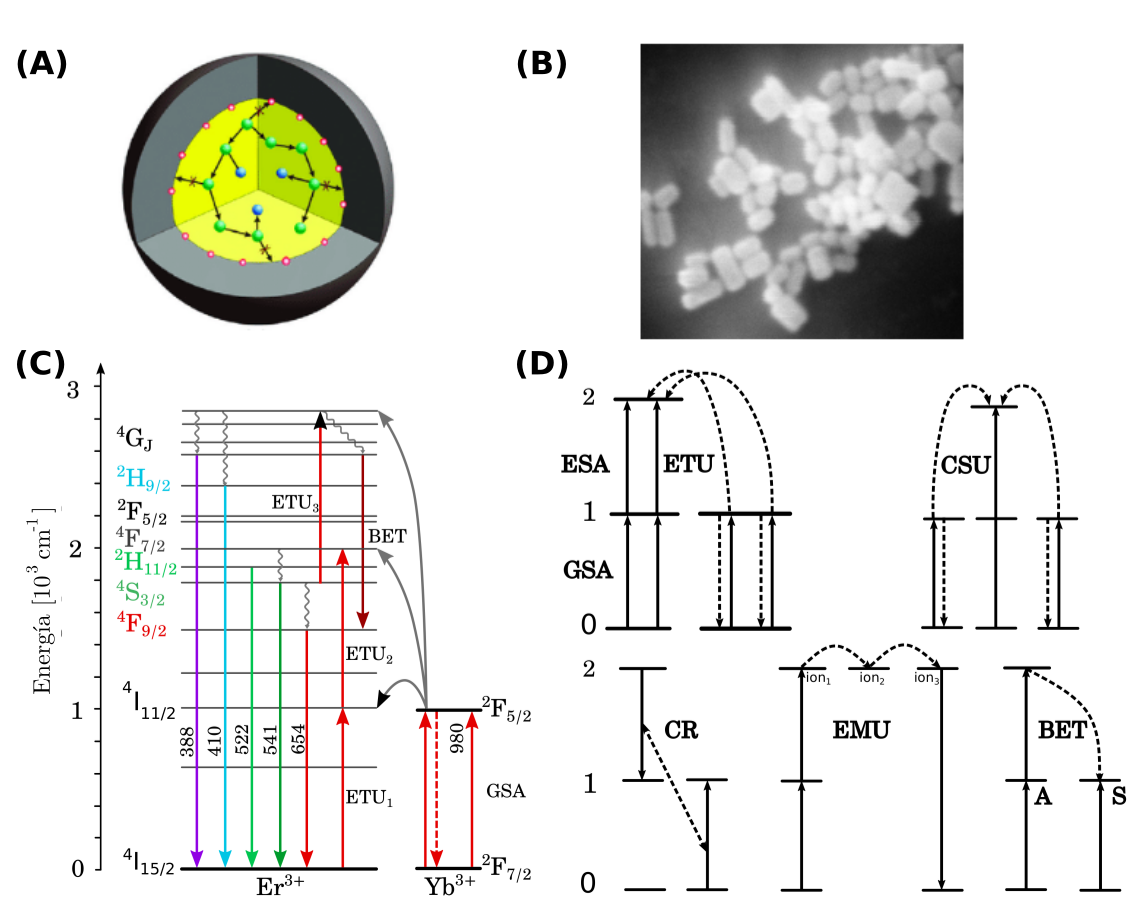
\includegraphics[width=\textwidth]{niveles_ucnp_imagen.png}
    \caption{\textbf{Diagrama de nanopartículas de \textit{upconversion}.} (\textbf{A}) Diagrama de una UCNP. Consiste en una matriz cristalina dopada con lantánidos en el interior (amarillo), y una capa externa (negro) sin dopaje. (\textbf{B}) Imagen SEM de las nanopartículas utilizadas durante esta tésis. (\textbf{C}) Diagrama de niveles de una UCNP dopada con iones de erbio Er$^{3+}$ e iterbio Yb$^{3+}$. (\textbf{D}) Mecanismos principales de interacción entre los dopantes. Tomada de \cite{bujjamer2020}.}
    \label{fig:ucnp_niveles}
\end{figure}

\subsection{Mecanismos y dinámica de las UCNP}

Para que la excitación sucesiva de los iones de erbio sea posible, distintos mecanismos de transferencia de energía se dan con el iterbio.
Un diagrama de cada uno de ellos se puede ver en la figura (\textbf{\ref{fig:ucnp_niveles}D}).
Todas las excitaciones comienzan por una excitación del nivel fundamental (\textit{Ground State Absorption}, GSA) al primero excitado en la escalera de niveles con energía de 980 nm.
Esto puede pasar tanto para el erbio como para el iterbio, pero como comentamos en la sección anterior, el iterbio tiene una sección eficaz mucho mayor, y por lo tanto es más probable que absorba un ion.
Una vez en el estado excitado, gracias a sus largos tiempos de vida, el Er tiene una probabilidad apreciable de volvera absorber otro fotón (\textit{Excited State Absorption}, ESA), excitandolo al nivel $^4$F$_{7/2}$ con energía equivalente a $\sim 490$nm.
Con menor probabilidad, la situación se podría volver a repetir.
Otra alternativa es que un ion excitado de Yb transfiera su energía de forma no radiativa a través de interacciones dipolo-dipolo a un ion de Er (\textit{Energy Transfer Upconversion}, ETU) \cite{Auzel2004}.
En este caso, el Yb vuelve a su estado fundamental sin emitir un fotón, y el Er excita su electrón de valencia a un nivel más alto.
Tanto ETU como ESA son los mecanismos más probables que causan la luminiscencia de las UCNP \cite{pollnau2000}.
\textit{Cooperative Sensitization Upconversion} (CSU) y \textit{Energy Migration Upconversion} (EMU) son mecanismos que requieren la interacción de tres iones, en los que los estados excitados se transfieren de unos a otros.
Algunos de los mecanismos, como la relajación cruzada (\textit{Cross Relaxation}, CR), no benefician la luminiscencia, sinó que la perjudican.
CR consiste en la interacción de dos electrones excitados en la que ambos quedan en un estado intermedio no radiativo.
\textit{Back Energy Transfer} (BET) es otro de este tipo, consiste en la relajación de un ion activador en un estado excitado a un sensibilizador \cite{bujjamer2020}.

Cada uno de estos mecanismos hace una contribución a la dinámica de la transición de estados de las UCNP.
A diferencia de los sistemas fluorescentes más simples como los discutidos en la sección \ref{sec:dinamica}, las ecuaciones dinámicas de las nanopartículas de \textit{upconversion} resultan en sistemas de ecuaciones más complejos.
Para empezar, hay una ecuación para cada nivel de energía excitado.
Además, cada mecanismo de transferencia agrega términos cruzados en las ecuaciones, y al depender de la presencia de fotones en más de un nivel, suelen ser términos no lineales.
Cada uno de esos términos también está acompañado por un coeficiente desconocido que describe el tiempo característico del mecanismo.
El resultado es un sistema de doce ecuaciones diferenciales ordinarias no lineales, con decenas de parámetros desconocidos \cite{anderson_revisiting_2014}.
Los términos no lineales de las ecuaciones dinámicas se asocian con la absorción secuencial de $n$ fotones que tiene que ocurrir para que las UCNP emitan luz.
Esto tiene una consecuencia directa en las observaciones de los experimentos: la luminiscencia depende de la densidad de potencia de excitación como una ley de potencias \cite{pollnau2000}.
Cada mecanismo sigue una ley de potencias con distinto exponente, pero tienen en común que están relacionadas con el número de fotones presente en el proceso.

\subsection{Requisitos para la caracterización óptica de las UCNP}

Las UCNP son un sistema luminiscente que convierte fotones de 980 nm en el NIR al espectro visible a través de múltiples interacciones entre los iones lantánidos que las componen.
Esta interacción se modela a través de un sistema de doce ecuaciones diferenciales no lineales con decenas de parámetros desconocidos.
La no linealidad del sistema implica que tanto los espectros como los tiempos de vida dependen de la densidad de potencia de excitación de forma no trivial.
Una caracterización óptica ideal de las nanopartículas requeriría ajustar los parámetros de este sistema, aunque esto resulta imposible a fines prácticos por el tamaño del espacio de parámetros y los largos tiempos de adquisición de cada experimento, especialmente a bajas potencias de excitación.

Un instrumento apropiado para caracterizar ópticamente las UCNP debería ser capaz de:

\begin{enumerate}
    \item Medir espectros estacionarios al excitar una muestra de forma continua.
    \item Medir tiempos de vida para los distintos picos de emisión de las partículas.
    \item Variar la potencia de excitación.
\end{enumerate}

\noindent Idealmente, el instrumento debería ser capaz de realizar mediciones de forma automática para paliar con los largos tiempos que requieren los experimentos.
En esta tésis tomamos un espectrofluorímetro antiguo Horiba PTI Quanta Master 400, lo renovamos y ampliamos sus capacidades para que cumpla con estos requisitos.
Luego, utilizamos el espectrofluorímetro renovado para caracterizar un lote de nanopartículas de \textit{upconversion} de NaYF$_4$:Er$^{3+}$,Yb${3+}$.

En el capítulo 2 describimos con detalle el \textit{hardware} del instrumento original, explicamos qué partes conservamos y cómo reemplazamos las partes que descartamos.
Posteriormente hacemos una caracterización del sistema de detección de fotones, tanto de la respuesta del \textit{hardware} como la detección de picos a través del \textit{software}.
En el capítulo 3 explicamos cuál es la estructura del \textit{software} que controla el instrumento, así como los protocolos que implementa para realizar una medición estática y una dinámica.
Por último, en la primera sección del capítulo 4 utilizamos el instrumento modificado para medir el espectro estático de excitación y emisión de una muestra patrón y lo comparamos con la misma medición hecha con el instrumento original.
En la segunda sección hacemos una caracterización óptica completa de un lote de las UCNP, midiendo sus espectros estáticos en función de la potencia, así como sus tiempos de vida para los picos de mayor emisión.




\chapter{Espectrofluorímetro para la caracterización de UCNPs}
\renewcommand{\tablename}{\textbf{Tabla}}

En este capítulo de la tésis se describe detalladamente la plataforma de fuente abierta que desarrollamos para renovar la electrónica y el \textit{software} de control del espectrofluorímetro Horiba PTI Quanta Master (QM 400), uno de los espectrofluorímetros antigüos del laboratorio de fotoquímica del INQUIMAE.
Además de su renovación, ampliamos sus capacidades para medir tiempos de vida del orden de los microsegundos, que junto con el agregado de un láser pulsado externo de 980 nm nos permitió conseguir la plataforma ideal para la caracterización óptica de UCNPs tanto estática como dinámica.


\section{Renovación y ampliación del fluorímetro Horiba PTI Quanta Master 400}

\subsection{Componentes originales}

La serie Horiba PTI QM incluye espectrofluorímetros modulares para investigación científica y sistemas optimizados para mediciones de fotoluminiscencia.
Estos espectrofluorímetros se encuentran frecuentemente en los laboratorios de Argentina, por ejemplo, sabemos que hay tres equipos de esta serie en el laboratorio de fotoquímica del INQUIMAE (QM400, QM-4 y RatioMaster), dos en el Centro de Investigaciones en Bionanociencias (CIBION) y uno en el Centro Atómico Constituyentes de la Comisión Nacional de Energía Atómica (CAC-CNEA), y probablemente haya más similares en otras instituciones.
Al ser modelos antigüos y descontinuados se pueden encontrar en el mercado por precios que rondan los \$5000 USD, un costo relativamente bajo para un espectrofluorímetro científico.
Los bajos costos se dan por su antigüedad y fin de soporte por parte de la empresa, lo que obliga a los usuarios a resolver ellos mismos los problemas que haya con los equipos.
Por ejemplo, en CIBION, uno de los dos modelos que tienen no está funcionando porque hay problemas con la inicialización de los controladores en la PC.
En este trabajo, reacondicionamos específicamente un espectrofluorímetro QM 400 de más de 30 años de antigüedad,  (diagrama en la \textbf{Fig. \ref{fig:ref-diagram}A} y fotografía en la \textbf{Fig. \ref{fig:hardware}A}), pero dada la similaridad entre los distintos modelos de esta serie, la renovación se pueden aplicar a cualquiera de ellos con leves modificaciones. 

El QM 400 está equipado con una lámpara de xenón de 75 W como fuente de luz, la cual proporciona un amplio espectro de longitudes de onda (desde el infrarrojo cercano, alrededor de 1000 nm, hasta el ultravioleta, alrededor de 300 nm).
Los monocromadores de excitación y emisión contienen redes de difracción rotadas por motores paso a paso de 200 pasos por revolución, con especificaciones de 7 V y 0.7 A por bobina (M1 y M2), lo que permite una resolución en la selección de longitudes de onda de 0.5 nm. 
Ambos incluyen un fin de carrera electromecánico para verificar si se ha alcanzado la longitud de onda máxima.
Los motores paso a paso, junto con sus fines de carrera respectivos, están conectados a un módulo controlador de motores (MDM) mediante conectores propietarios no documentados. 
Los fotones son detectados por un tubo fotomultiplicador (PMT, modelo PTI 810), cuya caracterización se detalla en la sección \ref{sec:caracterizacion_pmt}.
Éste está conectado al MDM a través de un cable BNC y polarizado con 1000 V desde una fuente de alimentación externa proporcionada también por el MDM. 
Esto genera pulsos negativos de alrededor de 170 ns con una terminación de 50 Ohm y un voltaje de −3.5 V (\textbf{Fig. \ref{fig:ref-diagram}D}). 
Finalmente, el MDM está conectado mediante un cable plano a una tarjeta de interfaz ISA en una PC con sistema operativo Windows 95 y el programa FelixGX, un \textit{software} propietario de adquisición y control instalado por Horiba (\textbf{Fig. \ref{fig:ref-diagram}B}).
FelixGX permite medir espectros de emisión y excitación (\textbf{Fig. \ref{fig:ref-diagram}E}), además de brindar herramientas de análisis rápido de los datos y controlar diferentes periféricos.

La antigüedad de la PC y electrónica de control hace que el proceso de adquisición de datos sea tedioso, y más aún para la caracterización de UCNPs.
Para hacer una medición el usuario debe colocar la muestra en la cámara y luego configurar en FelixGX un barrido de la longitud de onda de excitación o emisión.
En el caso de medir \textit{upconversion} se debe agregar un láser controlado externamente por una fuente de corriente (\textbf{Fig. \ref{fig:ref-diagram}A}) en la que se debe configurar por separado los parámetros de excitación, como la potencia.
Una plataforma de caracterización óptica completa de UCNPs debería ser capaz de medir espectros de emisión y tiempos de vida (del orden de los microsegundos) excitando a 980 nm con distintas densidades de potencia.
Además, como las mediciones de espectro y tiempo de vida son de larga duración (en especial a bajas potencias), resulta ideal que la plataforma permita configurar múltiples mediciones sucesivas sin la necesidad de una configuración manual por el usuario.
Durante su tésis de doctorado, Juan Bujjamer agregó la capacidad de medir tiempos de vida típicos de \textit{upconversion} al QM 400 \cite{bujjamer2020}. 
Para lograrlo utilizó en conjunto el control de los monocromadores que brinda FelixGX, una CPU y FPGA Red Pitaya y una fuente de diodo láser externa.
El excelente trabajo de Juan durante sentó las bases para que en este trabajo podamos hacer una renovación total del QM 400, utilizando como única plataforma de control a la Red Pitaya e independizandonos de la PC de control original.
En las siguientes secciones, explicaremos los cambios de \textit{hardware} y \textit{software} que realizamos en el espectrofluorímetro para que sea una plataforma ideal para medir \textit{upconversion}.



\begin{figure}[btp]
     \centering
     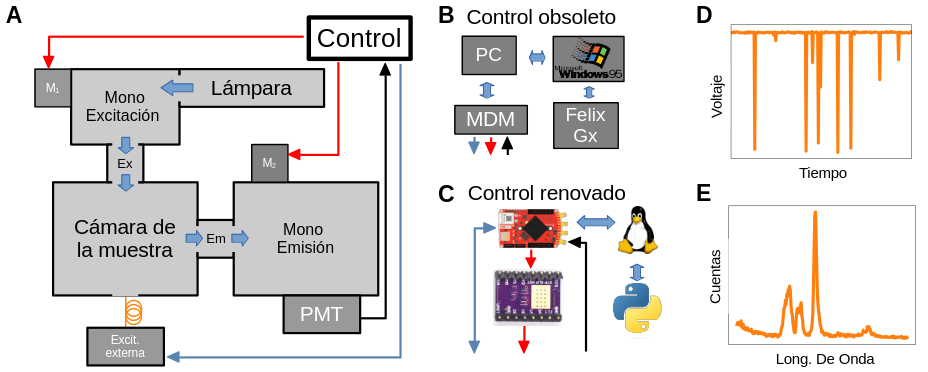
\includegraphics[width=\textwidth]{spec_diagram.png}
     \caption{
     \textbf{Representación esquemática del espectrofluorímetro}
     (\textbf{A}) Diagrama del hardware del Horiba PTI QM 400. Las flechas rojas representan los conectores de motores y fines de carrera, las negras corresponden a BNC, las azules a USB y las naranjas representan fibra óptica. La trayectoria de la luz dentro del espectrómetro está indicada con flechas azules gruesas.
     (\textbf{B}) y (\textbf{C}) Representación del módulo de control instrumental antiguo y nuevo, respectivamente.
     (\textbf{D}) Representación de la señal cruda medida por el detector PMT.
     (\textbf{E}) Espectro de la muestra construido a partir del conteo de picos en las señales crudas medidas para cada longitud de onda.
    }
     \label{fig:ref-diagram}
\end{figure}

\begin{figure}[h]
     \centering
     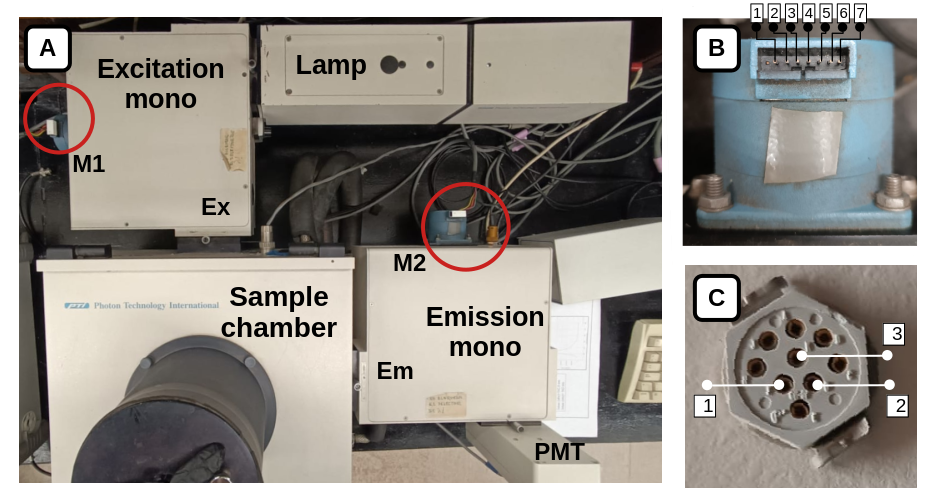
\includegraphics[width=0.9\textwidth]{hardware.png}
     \caption{\textbf{Foto del Horiba PTI Quanta Master 400}. 
    (\textbf{A}) Imagen del espectrómetro completo. En rojo se señalan los motores de los monocromadores y los fines de carrera. (\textbf{B}) Diagrama de pines de los motores paso a paso. Los únicos pines utilizados en la versión renovada son 1 y 7, y 3 y 5, que corresponden a cada bobina del motor respectivamente. (\textbf{C}) Diagrama de pines de los fines de carrera.}
     \label{fig:hardware}
\end{figure}



\subsection{Hardware para la renovación del QM 400}

\todo{pequeño parrafo de las partes en la que constó la cosa esta}

Luego de hacer una inspección de todas las partes, decidimos conservar los componentes ópticos, la motorización, el PMT, la fuente de alta tensión y el chasis, ya que son robustos y funcionales.  
En contraste, la electrónica de control y detección resultó ser voluminosa, de código cerrado y obsoleta, por lo que optamos por reemplazarla con alternativas modernas: una CPU con FPGA integrada Red Pitaya (RP) STEM LAB 125-14.
La RP cuenta con cuatro entradas y salidas analógicas que emiten y procesan señales en las radiofrecuencias, y un conjunto de pines digitales que permiten controlar circuitos integrados fácilmente.
Esta placa junto con dos circuitos integrados DRV8825 que simplifican el control de los motores por paso cumplen la tarea de controlar a los monocromadores.
Este cambio en la electrónica de control nos permitió reemplazar el voluminoso módulo MDM ($\sim$10 cm $\times$ 30 cm $\times$ 30 cm) por dos controladores DRV8825 soldados a una placa PCB mucho más pequeña (10 cm$\times$ 10 cm $\times$ 2 cm)(\textbf{Fig. \ref{fig:placa}}).
Para facilitar la conexión de los componentes del espectrofluorímetro a la RP también agregamos a la placa un puerto IDC que permite conectar los pines digitales, y conectores a los motores a través de fichas adaptadas a medida.
El PMT se conecta a través de un cable BNC-SMA a uno de los canales analógicos de radiofrecuencias de la RP, luego son digitalizados por su conversor analógico digital (ADC)(\textbf{Fig. \ref{fig:ref-diagram}D}) y luego contados por software (\textbf{Fig. \ref{fig:ref-diagram}E}).
Todas las conexiones se ven detalladas en la figura (\textbf{\ref{fig:connection_diagram}}).
El ADC de 14 bits de la RP se configura con una frecuencia de muestreo de 31.25 MHz de forma tal de satisfacer el criterio de Nyquist (ver sección \ref{sec:caracterizacion_pmt}).
RP tiene una interfaz de programación de aplicaciones que permite configurar dos métodos distintos para comenzar una adquisición de datos.
Una opción es llamar a una función que comienza la adquisición de inmediato.
Alternativamente, se puede configurar una de las entradas analógicas o digitales como \textit{trigger} para comenzar una medición.
Nosotros usamos el primer método para medir espectros estáticos y el otro para medir tiempos de vida.
Asimismo, la RP tiene dos mecanismos distintos para escribir los datos en la memoria al hacer una adquisición: un método por defecto de escritura a un espacio de memoria de 2$^{14}$ enteros de 16 bits, y un método de adquisición de memoria profunda (DMA) que permite guardar hasta 2 MB \cite{DMA_rp}.
Con esta capacidad para almacenar datos, a 31.25 MHz la ventana temporal de pulsos más grande que se puede obtener es de $\sim 0.5$ ms y $\sim 8$ ms respectivamente.
Aunque resulta beneficioso el método DMA y se podría implementar en esta renovación, nosotros utilizamos el método por defecto por la simplicidad que significó durante el desarrollo.
Para contrarrestar la corta duración de la ventana de adquisición, el software de control que desarrollamos permite agregar una demora para obtener ventanas de medición más grandes (ver sección \ref{sec:proceso_dinamico}).
El apéndice \ref{apendice:instrucciones_armado} explica detalladamente cómo reproducir las conexiones.

\begin{figure}
     \centering
     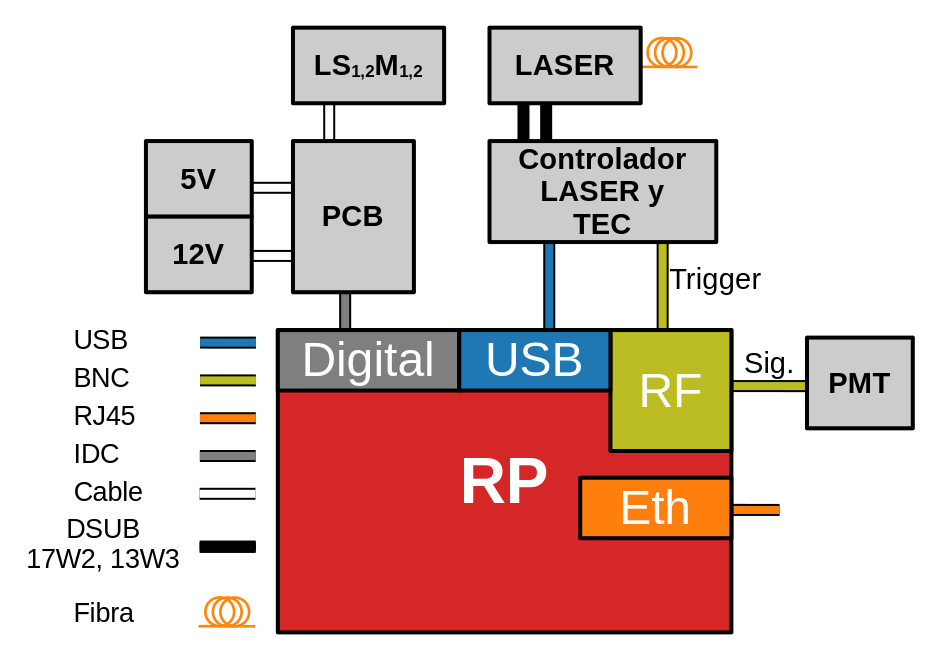
\includegraphics[width=0.8\textwidth]{connection_diagram.png}
     \caption{
    \textbf{Conexiones necesarias para la renovación y ampliación del QM400.}
    }
     \label{fig:connection_diagram}
\end{figure}



\subsection{Hardware ampliación}

El espectrofluorímetro original QM 400 disponible en el laboratorio no era adecuado para estudiar \textit{upconversion}, ya que no contaba con una fuente de luz en el infrarrojo (IR). 
Tampoco era posible realizar mediciones de tiempos de vida de la luminiscencia debido a la falta de excitación pulsada y detección dependiente del tiempo. 
Luego de aplicar renovación mencionada anteriormente, incorporamos estas funcionalidades al equipo y al \textit{software} de forma independiente.

Para ello, añadimos una fuente de luz IR externa modulable al sistema. 
En nuestro caso, utilizamos un controlador de diodo láser y temperatura (TEC) de banco THORLABS ITC4020, controlado por la RP, para operar un diodo láser BL976-SAG300 de 976 nm y 300 mW. 
La salida del diodo láser se conecta mediante una fibra óptica a la entrada de fuente externa del QM 400 (\textbf{Fig. \ref{fig:ref-diagram}A}). 
El ITC4020 permite configurar la frecuencia de pulsado y el ciclo de trabajo, además de proporcionar una señal TTL que está en 5 V cuando el láser está prendido y 0 V cuando está apagado.
Esta señal se conecta a otra de las entradas analógicas de la RP, que luego la utiliza como \textit{trigger} para sincronizar la finalización de la excitación del láser, con la medición de los pulsos eléctricos de los fotones.
Esa sincronización le permite al \textit{software} realizar histogramas y así medir los tiempos de vida, proceso que se explica en detalle en la sección \ref{sec:proceso_dinamico}.  


\begin{figure}[h]
     \centering
     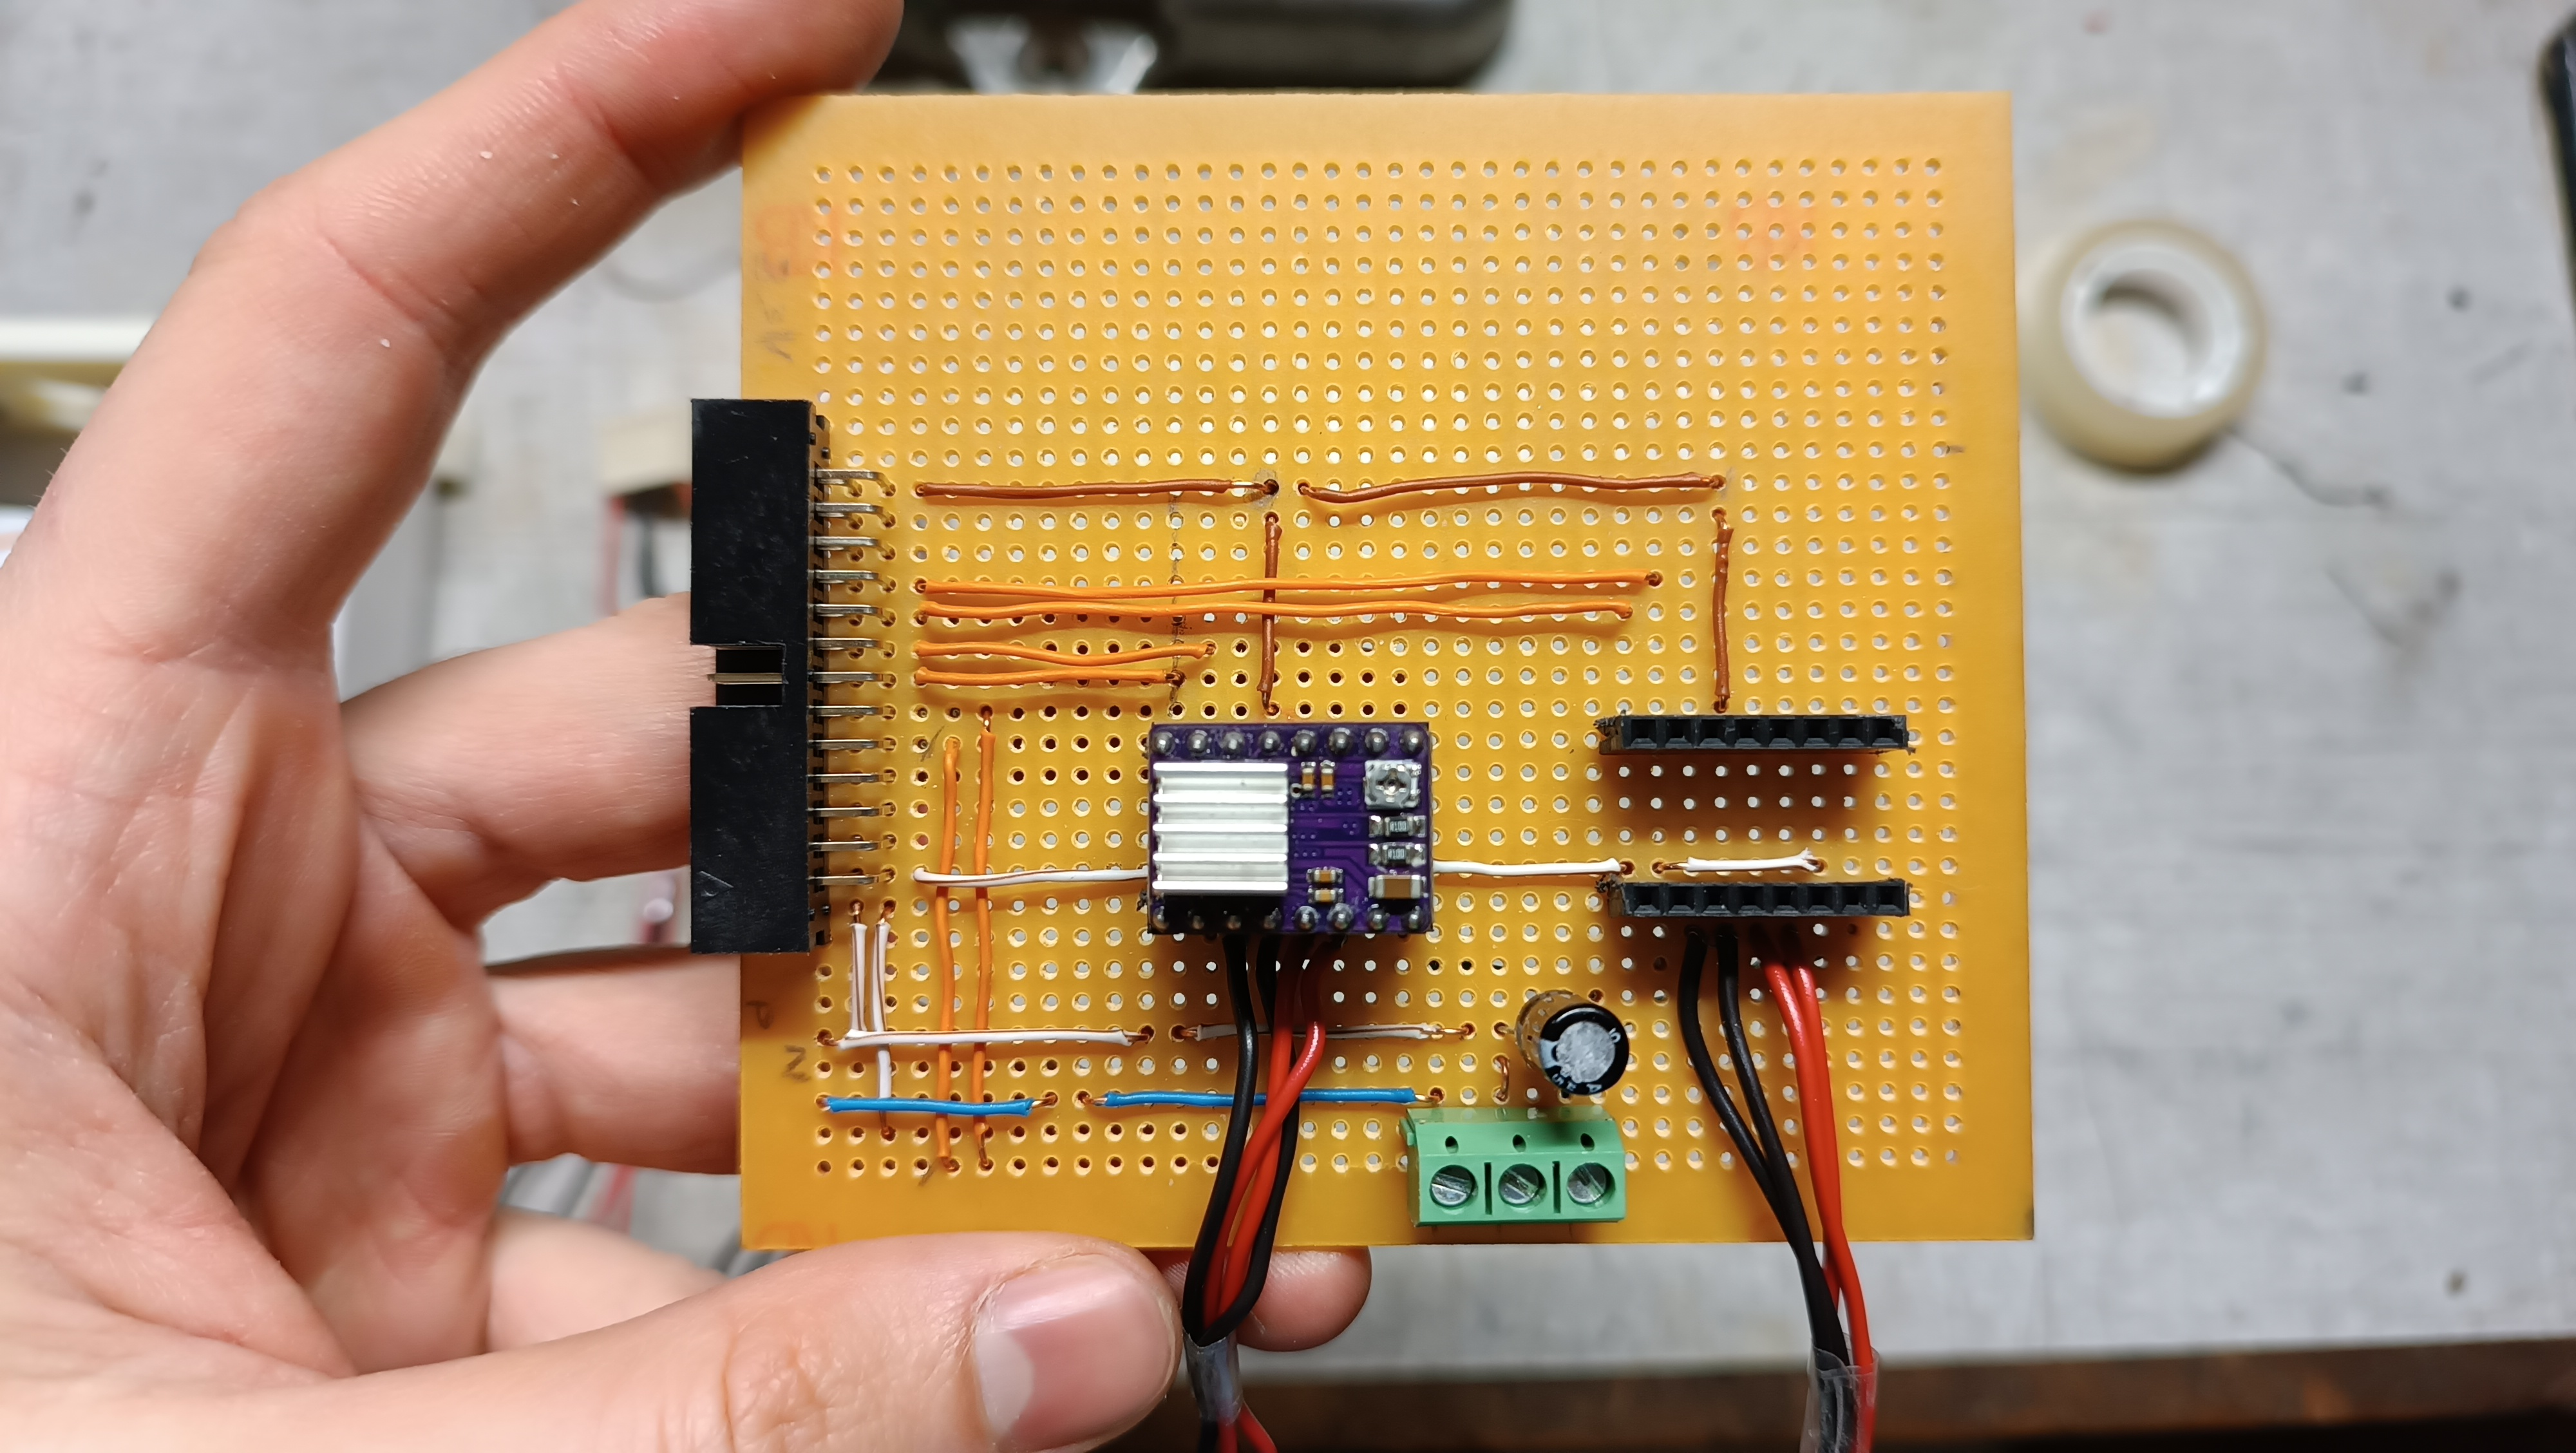
\includegraphics[width=0.9\textwidth]{placa.jpg}
     \caption{\textbf{Placa PCB con la electrónica de control.} La placa cuenta con un puerto IDC (izquierda) al que se conectan los pines digitales de la RP, que además provee la alimentación de 3.3 V a los circuitos integrados (centro). La placa incluye una bornera para proveer una referencia a tierra, una alimentación de 5 V y otra de 12 V.}
     \label{fig:placa}
\end{figure}


\section{Sistema de detección de fotones}


 
Los tubos fotomultiplicadores (PMTs) son detectores de fotones ampliamente utilizados en fluorómetros y cumplen un rol central en el funcionamiento del instrumento. 
Un PMT está compuesto por un fotocátodo y una serie de dínodos, que actúan como etapas de amplificación. 
Los fotones incidentes provocan la emisión de electrones desde el fotocátodo, y estos son amplificados sucesivamente por los dínodos. 
Al final del proceso, que tiene una duración típica de 40 a 50 nanosegundos, el pulso llega a un ánodo, desde donde se lee la señal. 
Este detector puede operar en dos modos: analógico o conteo de fotones. 
En el modo analógico, la corriente que fluye por el ánodo debe ser proporcional a la intensidad de luz que incide sobre el fotocátodo.
En el modo de conteo, el PMT registra pulsos eléctricos de corta duración cada vez que se detecta un fotón. 
Resulta crucial que el detector no se encuentre dañado, cosa que usualmente sucede por la exposición a luz muy intensa. 
Esto puede generar una corriente de oscuridad alta, pulsos espurios en la señal que sesgan el resultado de la medición \cite{lakowicz_principles_2006}.
En nuestro instrumento renovado, la señal del PMT se adquiere utilizando una Red Pitaya (RP). 
Este dispositivo permite una frecuencia máxima de adquisición de 125 MHz, aunque también es posible trabajar a frecuencias menores que sean divisiones por 2 de ese valor. 
Para realizar un conteo preciso de los fotones que inciden en el fotocátodo, caracterizamos la señal del PMT del QM 400 utilizando la RP en las mismas condiciones operativas del fluorímetro modificado.
Como resultado, medimos la corriente de oscuridad, determinamos el ancho medio de los pulsos y definimos el algoritmo de detección de pulsos más adecuado para optimizar el conteo. 
En las próximas secciones describimos en detalle esta caracterización.



\subsection{Caracterización del PMT con la Red Pitaya} \label{sec:caracterizacion_pmt}

\begin{figure}
    \centering
    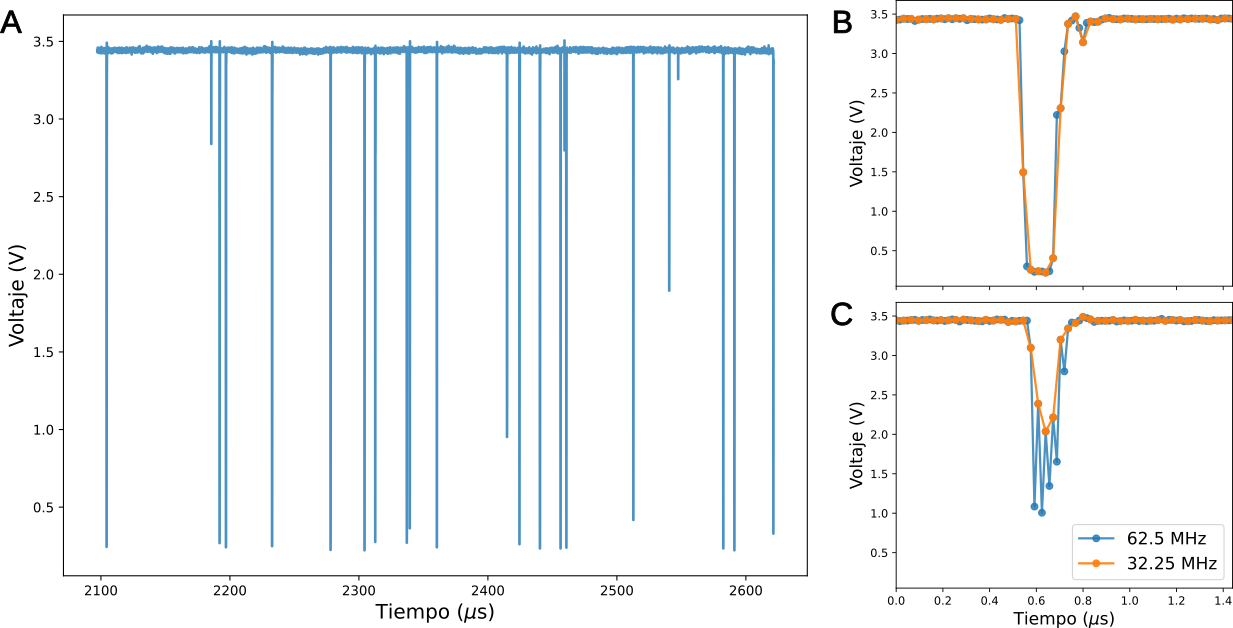
\includegraphics[width=\textwidth]{sig_pmt.png}
    \caption{\textbf{Señal del PMT.} (\textbf{A}) Medición de la señal del PMT en una ventana de la RP. Medidos a 62.5 MHz en azul y 31.25 MHz en naranja:(\textbf{B}) detalle de un pulso que satura al PMT, (\textbf{C}) Detalle de un pulso que no satura el PMT.}
    \label{fig:pmt_signal}
\end{figure}

Una señal típica del PMT al ser iluminado de forma constante, medida con una ventana de la RP a 31.25 MHz,  se puede ver en la figura (\textbf{\ref{fig:pmt_signal}A}).
La señal muestra un voltaje de base que ronda los 3.5 V, y múltiples picos negativos que representan la llegada de un fotón al fotocátodo.
Si bien la mayoría de pulsos suelen estar entre 1 y 0 V, hay otros que no llegan a saturar el detector y tienen menor altura.
Los pulsos que saturan tienen un tiempo rápido de subida, de aproximadamente $\sim 16$ ns, luego son constantes y después bajan rápidamente.  
Se puede notar una ligera asimetría en ellos, sus colas presentan dos rebotes alrededor de 2 y 3 V (\textbf{Fig. \ref{fig:pmt_signal}B}).
Por otro lado, los picos que no saturan presentan oscilaciones de alta frecuencia en el máximo.
Estos efectos se ven atenuados al medir a menores frecuencias de muestreo (\textbf{Fig. \ref{fig:pmt_signal}C}). 

La figura (\textbf{\ref{fig:histograma_puntos}}) muestra un histograma del voltaje de los puntos de una señal tomada con una frecuencia de muestreo de 31.25 MHz.
Para eliminar la base de la señal se tomaron sólo los puntos con voltajes menores a 3.4 V.
Se pueden ver dos picos en el histograma, uno para voltajes menores a 1 V, que corresponde a los pulsos que saturan al PMT, y otro para mayores a 3 V, que se pueden adjudicar al ruido y a los rebotes de la señal en las colas de los pulsos.
El eje vertical en escala logarítmica permite diferenciar un salto alrededor de 1.4 V, éste corresponde a los pulsos que no saturan y cuyas oscilaciones de alta frecuencia se ven atenuadas a 31.25 MHz.
Viendo el histograma de la altura de los pulsos, tomamos como criterio considerar un pulso de la señal como un fotón que llegó al detector a todos ellos cuyo pico sea menor a 1 V.
Además de esta medición a iluminación constante analizamos la señal sin iluminar, concluyendo que la corriente de oscuridad es suficientemente baja como para no considerarla en el conteo.

Para estimar el ancho promedio de los pulsos calculamos la autocorrelación a partir de la medición de múltiples ventanas de la señal del PMT bajo iluminación constante.
La relación entre la desviación estandar $\sigma$ de una distribución gaussiana, y la desviación estandar $\sigma_c$ su autocorrelación está dada por $\sigma = \sigma_c/\sqrt{2}$.
Aproximando a los pulsos que llegan al detector por gaussianos, y usando que el ancho total a mitad de altura (FWHM) de una gaussiana es FWHM $= 2 \sqrt{2 \ln{2}}\sigma$, podemos obtener el FWHM de los pulsos con la fórmula FWHM $= 2 \sqrt{2 \ln{2}}\sigma_c / \sqrt{2}$
Por lo tanto, ajustamos el resultado de las autocorrelaciones por una gaussiana y realizamos un histograma de las desviaciones estandar de los pulsos $\sigma = \sigma_c / \sqrt{2}$ obtenidas (\textbf{Fig. \ref{fig:ancho_pulsos}}).
Como resultado, el ancho temporal de los pulsos a mitad de altura es de $(\Delta t = 113 \pm 2)$ ns, donde definimos el error como dos desviaciones estándar de la media.
Esto nos permite definir una tasa máxima $R$ de fotones por segundo que podemos detectar con el PMT.
Bajo iluminación continua, la probabilidad de que un fotón llegue al detector en un tiempo $t$ al medir en un intervalo $T$ es uniforme.
Entonces, la probabilidad $P$ de que otro fotón se solape debe ser $P = R \times T$, por lo que si queremos que la probabilidad máxima sea del 90\%, podremos adquirir a una tasa de fotones por segundo de $R = P/T = 0.1/113 \times 10^9$ Hz$ = 8.9 \times 10^5$ Hz.

Las mediciones que mostramos en esta sección fueron útiles para determinar que un pulso de la señal es un fotón sólo si su máximo es menor a 1 V.
Además, nos permitieron limitar la tása máxima con la que se miden fotones a $R = 8.9 \times 10^5$ fotones por segundo para tener un 10\% de chances de que se solapen.

\begin{SCfigure}
    \centering
    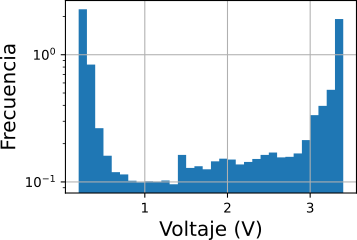
\includegraphics[width=0.5\textwidth]{histograma_puntos_pdf.png}
    \caption{\textbf{Histograma de voltajes} de una señal del PMT tomada con la RP a 31.25 MHz. El eje vertical está en escala logarítmica.}
    \label{fig:histograma_puntos}
\end{SCfigure}


\begin{figure}
    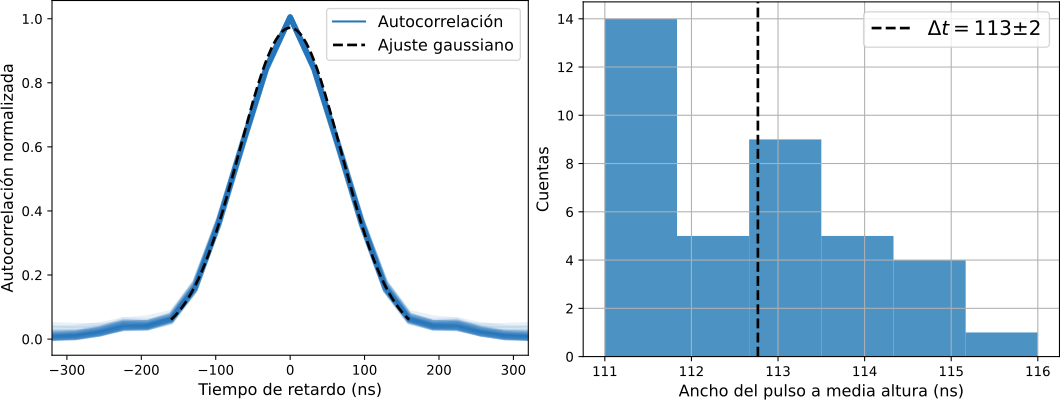
\includegraphics[width=\textwidth]{ancho_pulsos.png}
    \caption{\textbf{Autocorrelación} de las ventanas medidas por la RP a 31.25 MHz. A la izquierda se ve la autocorrelación de cada ventana y un ajuste gaussiano a una de ellas. A la derecha, un histograma de las desviaciones estandar de las gausianas.}
    \label{fig:ancho_pulsos}
\end{figure}

\subsection{Conteo de fotones} \label{sec:conteo}


Una vez que la RP obtiene la señal del PMT, el paso que queda para convertirla a intensidad lumínica es hacer un conteo de la cantidad de pulsos para la ventana de tiempo que midió.
Para esto, se necesita un algoritmo que tome como entrada la señal temporal del PMT $s(t)$, que muestreada es un conjunto discreto $\{s(t_i)\}$ y devuelva como salida el conjunto de tiempos $\{t_p\}$ en los que hay un pulso.
El algoritmo debe cumplir con dos condiciones: tiene que ser preciso para no sesgar los espectros y tiempos de vida, y tiene que ser rápido para que las mediciones se puedan hacer en tiempo real.

\begin{figure}
    \centering
    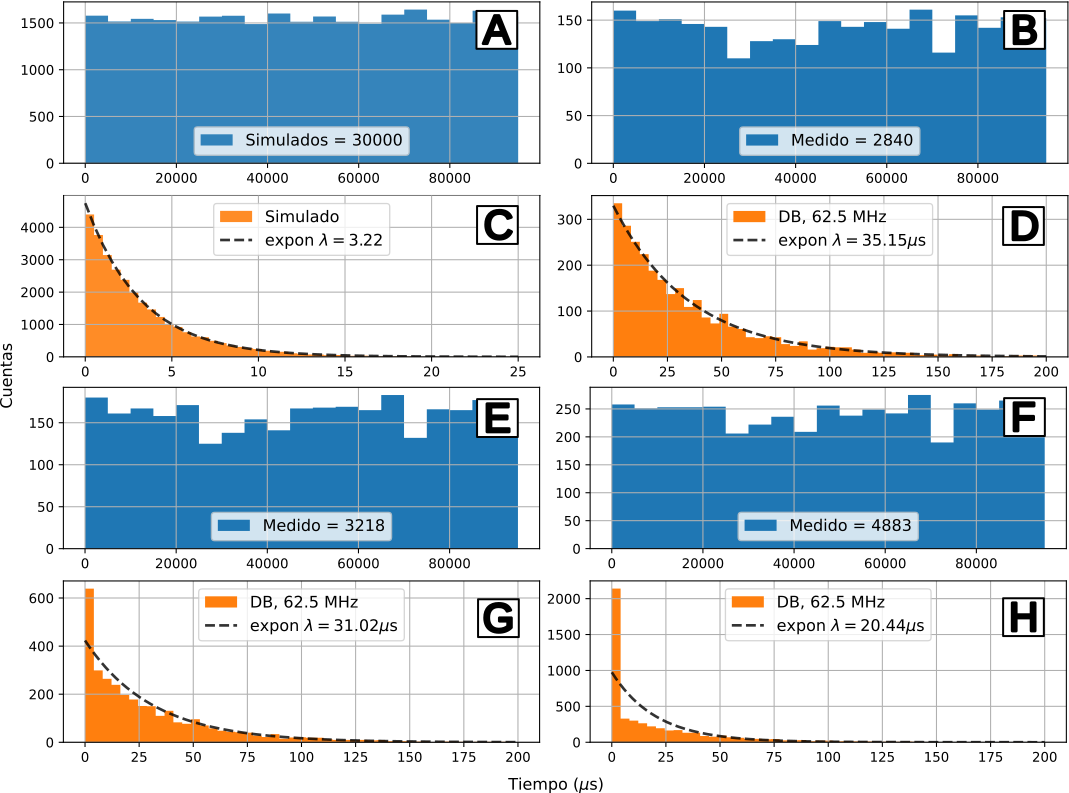
\includegraphics[width=\textwidth]{conteo.png}
    \caption{\textbf{Comparación de distintos métodos de conteo de fotones.} (\textbf{A}) distribución de pulsos simulados en un intervalo $T \sim 96$ ms y (\textbf{C}) distribución del tiempo $\Delta t$ entre esos pulsos. Análogamente, (\textbf{B}) y (\textbf{D}) para datos de pulsos medidos con frecuencia de muestreo de 31.25 MHz y detectados con el algoritmo $DB$. (\textbf{E}) y (\textbf{G}) medidos a 62.5 MHz y detectados con $DB$. (\textbf{F}) y (\textbf{H}) medidos a 31.25 MHz y detectados con $D$.}
    \label{fig:conteo}
\end{figure}

Nuestra implementación, que llamaremos DB, consiste en tres pasos, (i) binariza la señal temporal, (ii) busca los puntos en los que la derivada hace un salto y (iii) elimina los puntos que están muy cerca en el tiempo.
La binarización consiste en convertir en 1 a los puntos que sobrepasan (es decir, cuyo voltaje es menor que) cierto umbral $V_b$ y en 0 a los que no. 
Luego, se calcula la diferencia entre los puntos consecutivos $\Delta s(t_i) = s(t_{i+1}) - s(t_i)$, y se toma el conjunto $\{t_j\}$ en los que la diferencia es negativa.
Por último, se eliminan los puntos que estén a menos de $\Delta t_{min}$ de otros.
Si bien tanto $V_b$ como $\Delta t_{min}$ son configurables, los valores por defecto son $V_b = 1$V, que se tomó según lo encontrado en la sección \ref{sec:caracterizacion_pmt}, y $\Delta t_{min} = 0$, ya que vimos que cambiar este último valor no generaba una diferencia en los pulsos detectados.
Si bien existen otros algoritmos más sofisticados para encontrar picos, como la función \textit{find\_peaks\_cwt} del paquete de Python \textit{scipy}, estos suelen aplicar técnicas costosas computacionalmente, y por lo tanto lentas a comparación de tomar la derivada y binarización \cite{du_improved_2006}.

Una vez elegido el algoritmo, es necesario asegurarse que estuviera contando pulsos correctamente.
Para eso iluminamos una muestra con intensidad constante durante un intervalo $T$ de medición, calculamos la distribución de $\Delta t_j$ y la comparamos con una simulación equivalente (\textbf{Fig. \ref{fig:conteo}}).
La diferencia $\Delta t_i = t_{i+1} - t_i$ entre dos variables aleatorias uniformemente distribuidas, y ordenadas de forma tal que $t_1 < ... < t_i < t_{i+1} < ... < t_N $ es otra variable aleatoria con distribución exponencial y valor medio $T/N$, donde $N$ es el número de pulsos detectados \cite{dasuniform}.
La simulación consiste en N = 30000 pulsos uniformemente distribuidos en un intervalo de $\sim 96$ ms, lo que da un valor medio de $\lambda \equiv \langle \Delta t_j \rangle = 3.22$ $\mu$s (\textbf{Fig. \ref{fig:conteo}A y C}).
Se tomó N = 30000 para tener una buena estadística a la hora de comparar con la distribución de probabilidad exacta (línea punteada en \textbf{Fig. \ref{fig:conteo}C}) con el mismo valor medio.
Realizamos la medición por el mismo intervalo de tiempo con una frecuencia de muestreo de 62.5 MHz al iluminar una muestra con CW.
El algoritmo \textit{DB} detectó 3218 pulsos, y se ve que la distribución de $\Delta t_j$ parece seguir una exponencial excepto por el primer intervalo del histograma que tiene un número de cuentas mucho mayor que el resto (\textbf{Fig. \ref{fig:conteo}E y G}).
Esto se debe a las fluctuaciones de alta frecuencia, que hacen que \textit{DB} detecte dos $t_j$ para un mismo pulso de la señal. 
Para resolver este problema se puede aumentar $\Delta t_{min}$ o reducir la frecuencia de muestreo.
La frecuencia de 31.25 MHz sigue siendo capaz de detectar pulsos (ver \ref{sec:caracterizacion_pmt}), por lo que realizamos el mismo análisis sub-muestreando la señal original.
En este caso \textit{DB} detectó 2840 pulsos, y se ve que la distribución de $\Delta t$ sigue una exponencial con valor medio $\lambda = 68.12$ (\textbf{Fig. \ref{fig:conteo}B y D}).
A modo de comparación, también procesamos la señal a 31.25 MHz pero usando un algoritmo \textit{D} que consiste en tomar los puntos en los que la derivada es menor a un umbral (en este caso de -0.5).
Éste detectó 4883 pulsos, y se puede ver que también tiene el problema de detectar fluctuaciones de alta frecuencia, aumentando sintéticamente la cantidad de pulsos que hay en la señal (\textbf{Fig. \ref{fig:conteo}F y H}).

Por último, para tener una medida cuantitativa de la bondad de ajuste al modelo exponencial, calculamos el $\chi^2$ dado por la fórmula 

\begin{equation}
    \chi^2  = \sum_{i=1}^{n=50} \frac{(O_i - E_i)^2}{E_i},
\end{equation}

\noindent donde $n$ es el número de barras en el histograma, $O_i$ es la cantidad de cuentas observadas, y $E_i$ es la cantidad de cuentas esperadas, asumiendo que la distribución de los datos debería ser una exponencial con el valor medio observado $\langle \Delta t \rangle$.
Obtuvimos los estadísticos de la tabla \ref{tab:chisq}, donde el $\chi^2$ crítico es el correspondiente a un test de hipótesis con significancia $\alpha = 0.05$ \cite{frodesen_probability_1979}.
Después de esta comparación entre algoritmos de detección y frecuencias de sampleo, concluimos que la elección óptima es tomar los datos a 31.25 MHz y usar el algoritmo de detección \textit{DB}.

\begin{table}[t]
\centering
\begin{tabular}{|l|c|}
    \hline
    \textbf{Método} & \boldmath$\chi^2$ \\
    \hline
    DB 31.25 MHz & 48 \\
    D 31.25 MHz & 5690 \\
    DB 62.5 MHz & 486 \\
    Crítico & 65 \\
    \hline
\end{tabular}
\caption{Comparación del estadístico $\chi^2$ para los distintos métodos.}
\label{tab:chisq}
\end{table}



\chapter{Software y protocolos de medición}

\renewcommand{\tablename}{\textbf{Tabla}}

\section{Software} \label{sec:software}

Para reemplazar el rol que cumplía el \textit{software} FelixGX en el espectrofluorímetro original desarrollamos dos paquetes de Python de control de instrumental y adquisición de datos \cite{napoli_tdinapoli_2024,grecco_hgrecco_2024}.
El código corre en la CPU de la RP y permite controlar al espectrofluorímetro a través de una interfaz de programación de aplicaciones (API) y una interfaz gráfica simple (GUI) desarrollada con el paquete \textit{Jupyter Widgets} de \textit{IPython}.
El programa conformado por ambos paquetes está compuesto de cuatro capas principales (\textbf{Fig. \ref{fig:code}}):

\begin{itemize}
     \item \textbf{RedpiPy}: Es uno de los dos paquetes que desarrollamos. Consiste en un \textit{wrapper} (llamado \textit{rpwrap}) de la API original de la RP que resulta en que el código esté mejor organizado para hacer una aplicación en Python. Se compone de funciones y clases que permiten manejar el \textit{hardware} de la RP a bajo nivel, como \textit{RPDO} que controla los pines digitales, así como algunas clases de más alto nivel como \textit{Oscilloscope} que permite manejar el osciloscopio.
     \item \textbf{Clases de dispositivos}: Controlan componentes individuales del espectrofluorímetro, como los monocromadores, el láser pulsado, y los motores de los monocromadores permitiendo el control de todas las partes por separado. 
     \item \textbf{Clase Spectrometer}: Coordina el \textit{hardware} para protocolos de medición específicos (por ejemplo, adquirir un espectro de emisión). Es fácil de usar desde un script en Python o desde la línea de comandos. Además, es la encargada de contar los pulsos de voltaje negativo registrados por el PMT (ver sección \ref{sec:conteo}). Es utilizada por la interfaz gráfica.
     \item \textbf{Interfaz gráfica (GUI)}: proporciona herramientas de adquisición similares a las de FelixGX. Se accede a través de la web y utiliza el paquete \textit{Jupyter Widgets} de \textit{IPython}.
\end{itemize}

Gracias a este diseño la parte del código que implementa el control del instrumento es completamente general y está desacoplada del resto, por lo que debería funcionar para cualquier modelo de espectrofluorímetro cuyos monocromadores sean controlados por motores por paso, y la señal de luminiscencia se lea con un PMT.
Por otro lado, la API pública le permite al usuario avanzado crear sus propios protocolos de medición que se pueden ejecutar sin la supervición de un operario.
Tanto \textit{RedpiPy} como \textit{RefurbishedPTI} (el paquete que controla al espectrofluorímetro) se encuentran públicos en repositorios de \href{https://github.com}{GitHub} con sus respectivas instrucciones de instalación. 
El apéndice \ref{apendice:instrucciones_uso} explica detalladamente algunos ejemplos que muestran cómo medir un espectro estacionario y el tiempo de vida para distintas longitudes de onda, ambos a través de la API y de la GUI.
En las próximas secciones explicaremos cuál es el protocolo del software para hacer mediciones espectrales estáticas y dinámicas, independientemente de la interfaz que se use para obtenerlas.



\begin{figure}[t]
     \centering
     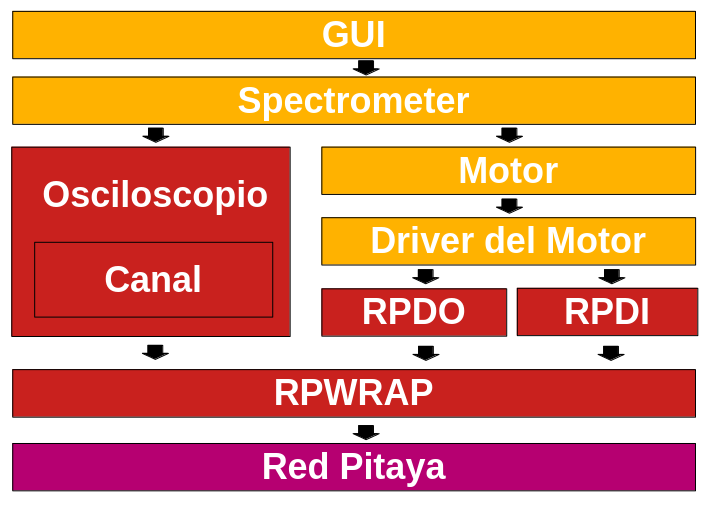
\includegraphics[width=0.8\textwidth]{software-diagram.png}
     \caption{\textbf{Estructura del \textit{software}}. Cada elemento del \textit{software} está ordenado de alto nivel (arriba) a bajo nivel (abajo). En amarillo se ven las componentes de \textit{refurbishedPTI}, en rojo las de \textit{redpipy}, en rosa la API y el \textit{hardware} de la RP.}
     \label{fig:code}
\end{figure}

\section{Protocolo de medición estática}

El espectro estático de emisión de una muestra consiste en la medición de su intensidad de luminiscencia al iluminar en una longitud de onda fija, y observar barriendo un rango de longitudes de onda.
La medición del espectro de excitación es análoga, pero cambia el rol de los monocromadores: en vez de observar la emisión en un rango de longitudes de onda, se observa en una longitud de onda fija y se barre un rango de longitudes de iluminación.
Por lo tanto, en el espectro de emisión, el monocromador estático es el de exctiación, y viceversa.
A continuación se detalla el protocolo de medición para un espectro de emisión estático.

Antes de iniciar una medición deben estar definidos sus parámetros que en este caso son el tiempo de integración $t_{int}$, la longitud de onda de iluminación $\lambda_e$ (la $e$ es por estático), y la longitud de onda inicial $\lambda_i$ y final $\lambda_f$ del barrido, así como el paso $\lambda_s$ entre cada medición de intensidad.
En el caso de tomar un espectro de UCNPs, dado que la iluminación proviene del diodo láser de 976 nm, también es necesario configurar la potencia óptica de excitación.

Una vez configurados los parámetros, el espectrofluorímetro debe realizar los siguientes pasos:

\begin{enumerate}
     \item \textbf{Inicializar los monocromadores} haciendo girar los motores en una misma dirección hasta que la señal del fin de carrera de cada uno sea de 5 V. Esto sirve para que la longitud de onda guardada por el \textit{software} coincida con la real.
     \item \textbf{Mover el monocromador estático} de emisión hasta $\lambda_e$. 
     \item \textbf{Mover el monocromador dinámico} de excitación hasta $\lambda_f$ en pasos de $\lambda_s$. Para cada longitud de onda los pasos (a) y (b) se deben repetir  $n$ veces, donde $n$ es tal que $n \times t_{max} \geq t_{int}$ y $t_{max}$ es el máximo tiempo de medición que soporta la RP (0.5 ms):
     \begin{enumerate}
          \item Medir la señal del PMT (\textbf{Fig. \ref{fig:diag_medicion_estatica}A}).
          \item Contar los picos en esa señal (ver sección \ref{sec:conteo}) y acumularlos. Al finalizar, el resultado es la cantidad de picos (fotones) contados por segundo.
     \end{enumerate}
\end{enumerate}

\noindent Una vez que el monocromador dinámico llega a $\lambda_f$ la cantidad de cuentas por segundo para cada longitud de onda se guarda en una tabla y termina la medición.
Al caracterizar UCNPs la excitación se da a través del láser externo, por lo que se deben configurar sus parámetros independientemente y el monocromador de excitación, que selecciona la longitud de onda de la lámpara que ilumina a la muestra, no toma ningún rol.
Como siempre se miden pantallas enteras, los tiempos de integración posibles son múltiplos de 0.5 ms.
Esto no es un problema porque los tiempos de integración necesarios suelen ser típicamente del orden de los segundos, dos o tres órdenes de magnitud mayores a la duración de la pantalla.
Además, la tabla de datos resultante de una medición contiene el tiempo de integración para cada punto con un error de $\sim 15$ ns.
En caso de que sea necesario medir con un tiempo de integración más preciso, esto se puede lograr modificando levemente el \textit{software} de \textit{refurbishedPTI}.

\begin{SCfigure}
     \centering
     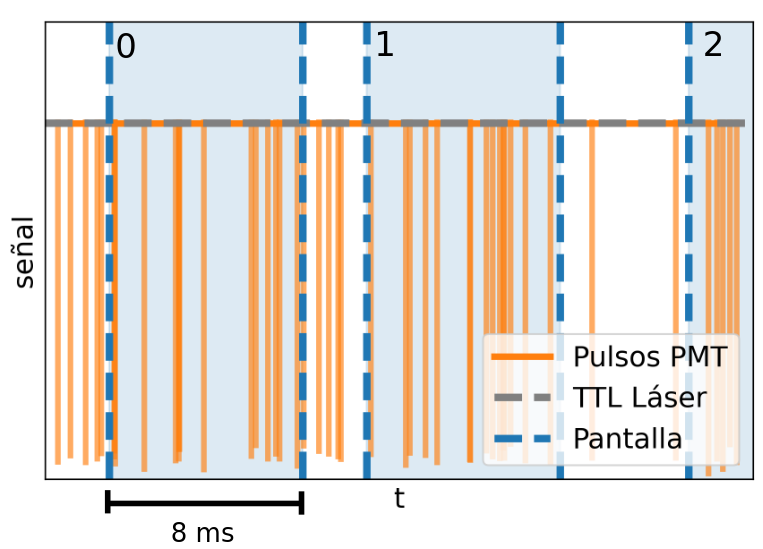
\includegraphics[width=0.6\textwidth]{diag_medicion_estatica.png}
     \caption{\textbf{Diagrama de medición estática.} En naranja se ve la señal del PMT. La línea punteada gris alta indica que el láser está en modo CW. En azul se ven las ventanas de la señal que lee la RP.}
     \label{fig:diag_medicion_estatica}
\end{SCfigure}


\section{Protocolo de medición dinámica} \label{sec:proceso_dinamico}

La medición de los tiempos de vida de las nanopartículas de \textit{upconversion} se realiza mediante la técnica de TCSPC (ver sección \ref{sec:intro_tcspc}).
Dado que estos tiempos de vida están en el rango de cientos de microsegundos, no son necesarios varios de los componentes de electrónica rápida típicos de la TCSPC utilizada en mediciones en el rango de nanosegundos, como el CFD y el TAC, los cuales son reemplazados por componentes más simples y menos costosos.
Contradictoriamente, esto hace que no se puedan caracterizar UCNPs utilizando equipos de fluorescencia de uso general, dado que el tiempo total de adquisición necesario difiere en órdenes de magnitud.
En nuestro caso, llevamos a cabo la técnica utilizando el trigger configurable a través de las entradas analógicas de la RP, y la señal TTL proveniente de la fuente de alimentación del láser.
Otra diferencia con TCSPC tradicional es el modo de excitación de la muestra.
Como la mayoría de fluoróforos orgánicos presentan su luminiscencia a través de la excitación de transiciones dipolares eléctricas, pérdia de energía por fonones, y re-emisión a través de otra transición dipolar, todos fenómenos que ocurren en el orden de los nanosegundos, es posible estudiar su espectro dinámico al excitar con un pulso del láser.
En el caso de las UCNPs, su luminiscencia se da por la dinámica no lineal de la interacción entre sus dopantes lantánidos (Yb$^{+3}$ y Er$^{+3}$), procesos que incluyen la excitación sucesiva sus electrones y por lo tanto ocurren en el orden de los microsegundos.
Por este motivo, es necesario iluminar a la muestra por algunos milisegundos para asegurarse de llegar al estado estacionario del sistema antes de medir su decaimiento.
Esto se hace aprovechando la función de alimentación pulsada (\textit{Quasi Continuous Wave} ó QCW) que ofrece la fuente ITC4020, la cual permite configurar frecuencia de pulsado $\nu$, y ciclo de trabajo $dc$ (\textbf{Fig. \ref{fig:diag_medicion_dinamica}}).

\begin{figure}
     \centering
     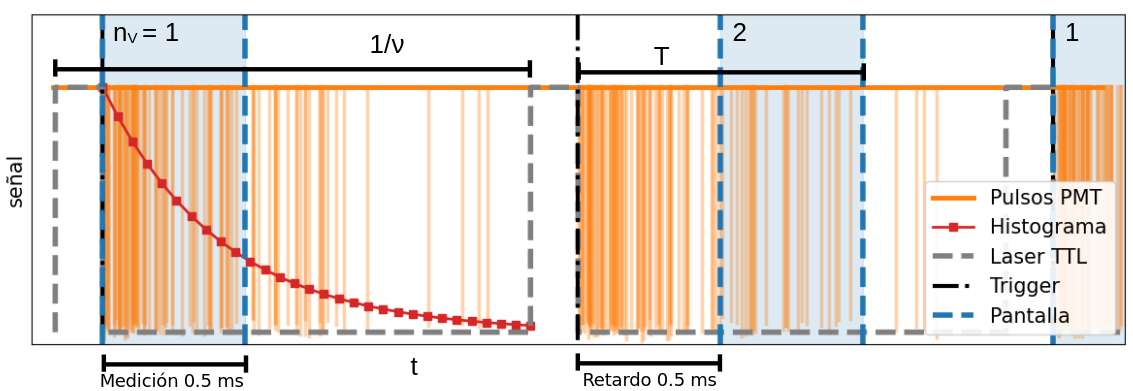
\includegraphics[width=\textwidth]{diag_medicion_dinamica.png}
     \caption{\textbf{Diagrama de medición dinámica.} La muestra es excitada intermitentemente con el láser (gris punteado). Al apagarse, el trigger de la RP se ejecuta y comienza a medir (azul) la señal (naranja) luego de esperar por $t_{ret}$. El resultado es un histograma (rojo) con la cantidad de fotones que llegaron en cada intervalo de tiempo.}
     \label{fig:diag_medicion_dinamica}
\end{figure}

Para hacer una medición de TCSPC es necesario definir la longitud de onda $\lambda$ en la que se detectará la emisión, el intervalo de tiempo $T$ en el que se van a contar los fotones luego del trigger, y la cantidad de veces $N$ que se va a medir ese intervalo.
Alternativamente, se podría definir un número de fotones $N_{fot}$ al que se quiere llegar, y medir el intervalo $T$ hasta que la cantidad de fotones medidos $n$ sea mayor a $N_{fot}$.
El protocolo por defecto de nuestro \textit{software} requiere determinar $N$.
Además, el intervalo de tiempo $T$ en el que se mide después del \textit{trigger} debe ser un múltiplo del tiempo máximo que puede medir la RP por ventana, $t_{max} = 0.5$ ms.
Por este motivo, en vez de especificar $T$, vamos a especificar $N_V$, el número de ventanas que queremos medir después del \textit{trigger} (\textbf{Fig. \ref{fig:diag_medicion_dinamica}}).
Entonces, el protocolo para realizar la medición es:

\begin{enumerate}
     \item \textbf{Inicializar los monocromadores} de forma análoga a la explicada en la sección anterior.
     \item \textbf{Mover el monocromador} de emisión hasta $\lambda$.
     \item \textbf{Iniciar el láser en modo QCW} y configurarlo para que se prenda y se apague con frecuencia $\nu$ y ciclo de trabajo $dc$.
     \item \textbf{Configurar la RP} para que espere un trigger en el canal analógico adecuado antes de medir.
     \item \textbf{Configurar un tiempo de retardo} $t_{ret} = (n_v - 1) \times t_{max}$, donde $1 \leq n_V \leq N_V$. $t_{ret}$ es el tiempo que la RP pasa sin medir después del \textit{trigger} para poder mover la ventana de medición (\textbf{Fig. \ref{fig:diag_medicion_dinamica}}). Repetir $N$ veces:
     \begin{enumerate}
          \item \textbf{Adquirir una ventana} después del \textit{trigger} y $t_{ret}$.
          \item \textbf{Encontrar los tiempos de llegada} de los pulsos usando el algoritmo explicado en la sección \ref{sec:conteo} y acumularlos.
     \end{enumerate}
     Al finalizar, el resultado es una tabla con los tiempos en los que llegaron los fotones después del \textit{trigger}.
\end{enumerate}

Con la tabla de datos final se construye un histograma (\textbf{Fig. \ref{fig:diag_medicion_dinamica}}), al cual se le puede ajustar un modelo de decaimiento para obtener el tiempo de vida de las partículas.


\chapter{Caracterización de UCNPs}


En este capítulo, vamos a utilizar el Horiba PTI QM 400 renovado y con su ampliación de capacidades para realizar mediciones de espectros estáticos de excitación y emisión, así como mediciones de tiempo de vida.
En la primera sección vamos a medir y comparar los espectros estacionarios de la rodamina B usando el instrumento renovado y el original.
En la segunda sección vamos a caracterizar ópticamente un lote de UCNPs.
Todas las partículas usadas en este trabajo fueron sintetizadas por el equipo colaborador del INQUIMAE, liderado por Beatriz Barja y María Claudia Marchi. 
Las nanopartículas utilizadas consisten en una red cristalina de fluoruro de ítrio NaYF$_4$ dopadas con los lantánidos iterbio (Yb) y erbio (Er), que en conjunto conforman una de las UCNPs más eficientes descriptas hasta el momento NaYF$_4$:Yb$^{+3}$,Er$^{+3}$ \cite{caracterizacion_ucnps_unicas}.
El método de síntensis empleado escapa el alcance de esta tésis, pero está detalladamente documentado en la literatura \cite{Zhang2012}.

\section{Espectros estacionarios de la rodamina B}

La rodamina es un fluoróforo extensamente usado en microscopía de fluorescencia debido a su fotoestabilidad y sus propiedades fotofísicas \cite{beija_synthesis_2009,rodamina_caracterizacion}.
Debido a su popularidad, sus espectros de excitación y emisión así como sus métodos de síntesis son ampliamente conocidos y reproducibles.
En particular, se caracteriza por tener un pico en 551 nm para la absorción y uno en 576 nm para la emisión.
A modo de verificación de que la medición de un espectro estático, tanto de excitación como de emisión, es el mismo utilizando el \textit{software} y el \textit{hardware} renovado y el original, medimos el espectro de la rodamina B.
Para eso Marcos Illescas, integrante del grupo de fotofísica del INQUIMAE, preparó una muestra de rodamina B disuelta en etanol.
Dado que el objetivo es comparar el espectro medido con el instrumento original y el renovado no se registraron las concentraciones ni la pureza de la solución.
La muestra se colocó en una cubeta y luego en el portacubetas de la cámara de muestras del fluorímetro.
Para el espectro de emisión se realizó la excitación con la lámpara de xenón original del instrumento a una longitud de onda fija de 520 nm y un barrido de emisión entre 530 y 700 nm.
Para el espectro de excitación se realizó un barrido de 420 a 590 nm, observando la intensidad de luz emitida a 600 nm.


En la figura (\textbf{\ref{fig:rodamina}}) se ven los cuatro espectros normalizados por su máximo de intensidad.
Se puede ver que los espectros medidos con el instrumento original (azul) se solapan completamente con los medidos con nuestra renovación (naranja).
Dado que las transiciones electrónicas presentes en la rodamina son dipolares sus tiempos de vida medios son del orden de los nanosegundos, por lo que son imposibles de medir con nuestro instrumento con resolución mínima de $\sim 100$ ns.
En la siguiente sección utilizamos el espectrofluorímetro renovado para su propósito inicial: la caracterización óptica de UCNPs.

\begin{SCfigure}
    \centering
    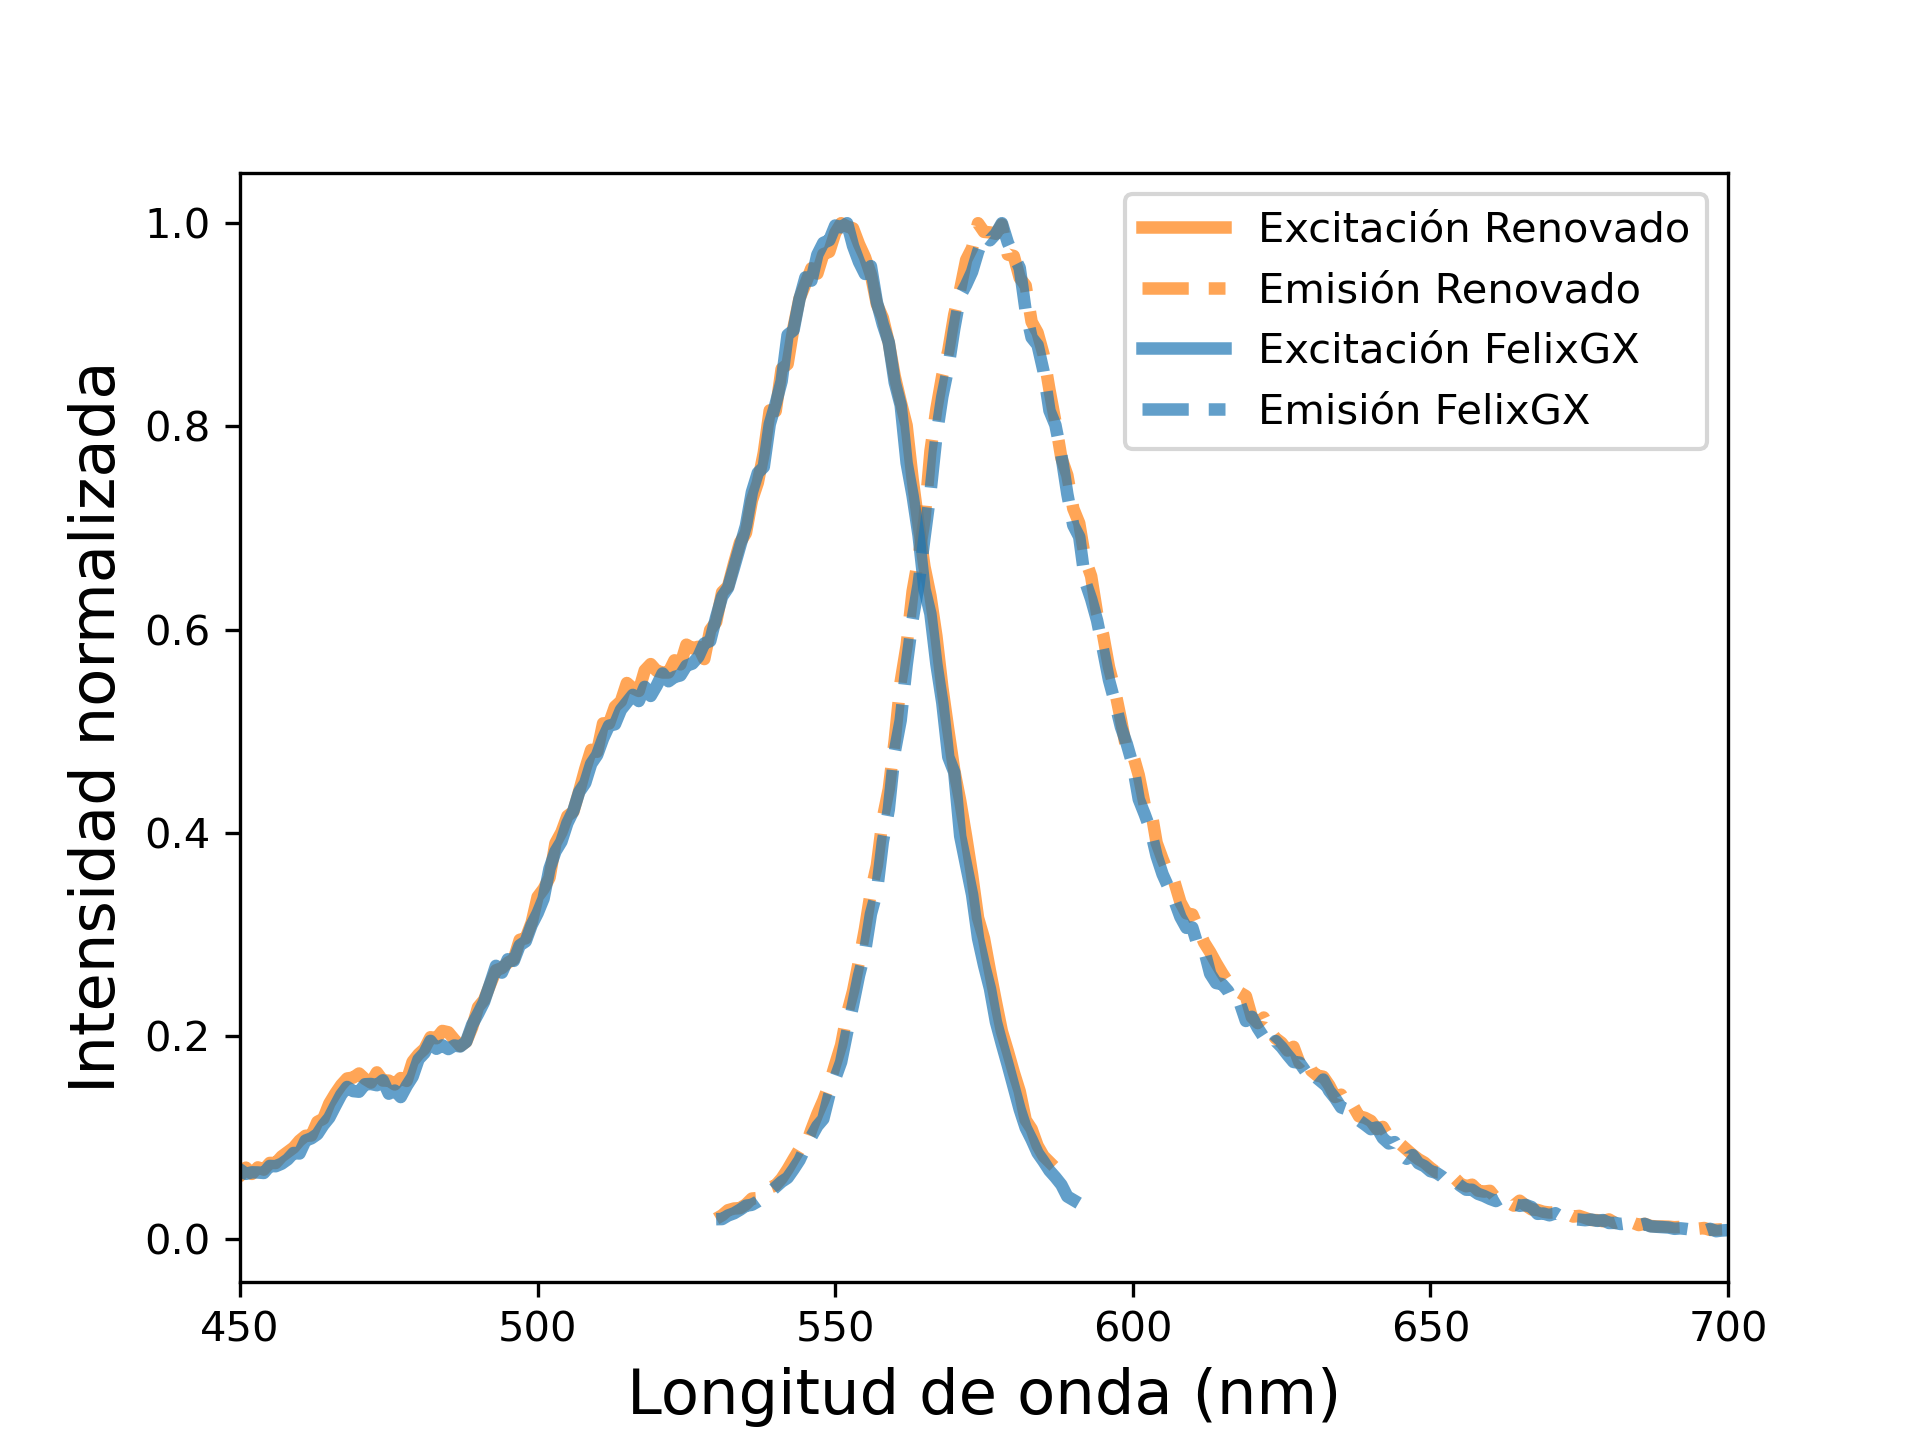
\includegraphics[width=0.7\textwidth]{rho6b_validacion.png}
    \caption{\textbf{Espectros de la rodamina B}, tanto de excitación (punteado) como de emisión (sólido). Ambos fueron medidos con el \textit{software} y \textit{hardware} original (azul) como con el renovado (naranja).}
    \label{fig:rodamina}
\end{SCfigure}

\section{Caracterización óptica de UCNPs}

\begin{figure}
    \centering
    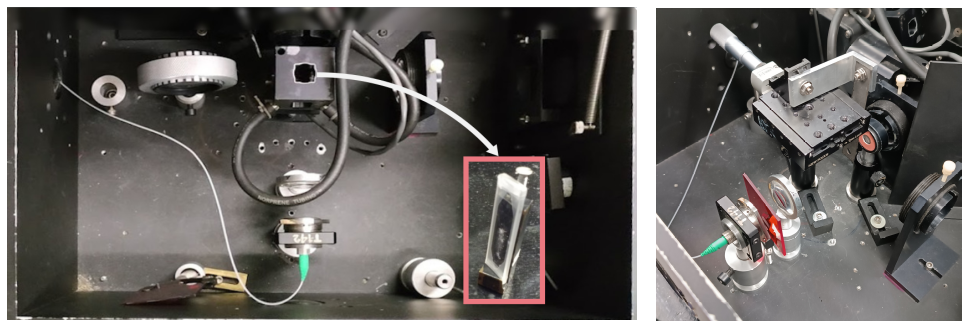
\includegraphics[width=\textwidth]{camara_muestra.png}
    \caption{\textbf{Imagen de la cámara de la muestra}. (izquierda) Se ve la cámara del fluorímetro sin filtro. Recuadrado en rosa hay una foto de la muestra sobre el sujetador. (derecha) Se ve el arreglo para medir el perfil del haz. En esta foto se ve el filtro utilizado en las mediciones.}
    \label{fig:camara_muestra}
\end{figure}

\begin{figure}
    \centering
    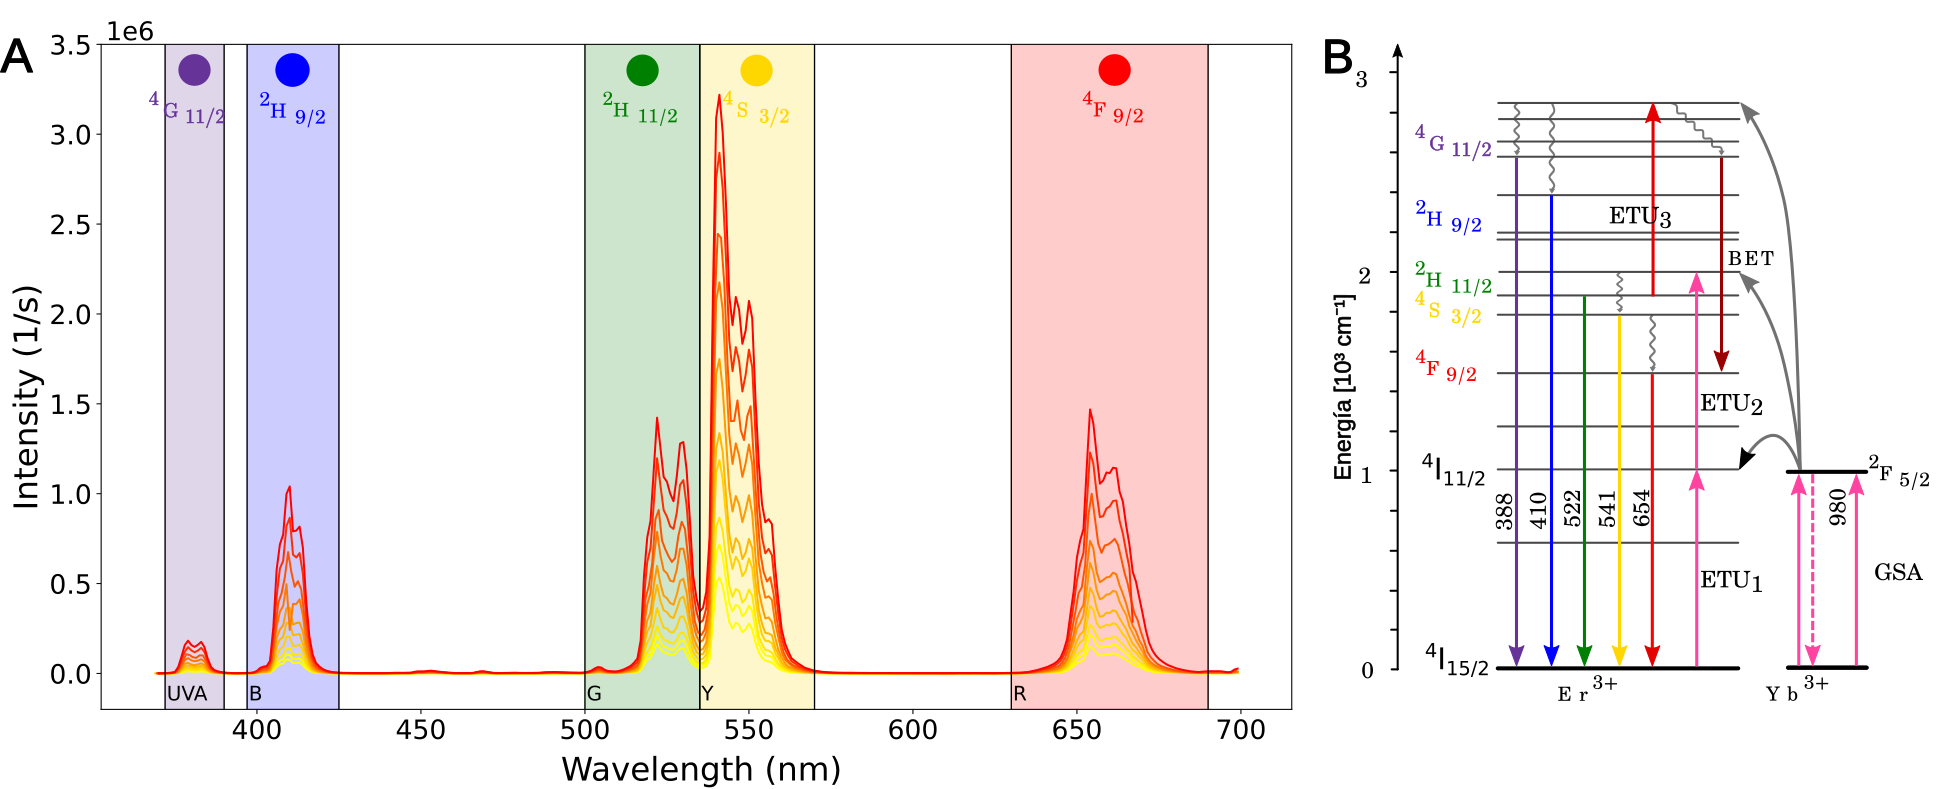
\includegraphics[width=\textwidth]{spectrum_powerdens.png}
    \caption{\textbf{Espectro de las UCNPs dependiente de la potencia.} (A) Espectro de emisión bajo excitación CW por un diodo láser de 976 nm para distintas densidades de potencia de excitación entre 16 mW cm$^{-2}$ y 80 mW cm$^{-2}$.
    (B) Esquema de niveles de Yb$^{+3}$ y Er$^{+3}$, marcados con colores los niveles excitados del Er$^{+3}$ cuya emisión corresponde a las regiones del espectro.}
    \label{fig:power_dep_spectrum}
\end{figure}

Nuestra plataforma adaptada nos permitió medir el espectro dinámico dependiente de la potencia de las UCNPs sintetizadas (\textbf{Fig. \ref{fig:power_dep_spectrum}}), y sus tiempos de vida (\textbf{Fig. \ref{fig:lifetimes}}) al ser excitadas con un láser de diodo IR de 976 nm.  
La muestra utilizada consta de un polvo de UCNP depositado sobre un portamuestras.
Sostuvimos al portamuestras con un sujetador que luego se coloca en el portacubetas de la cámara (\textbf{Fig. \ref{fig:camara_muestra}}).
El láser externo se acopla a fibra y luego se enfoca con una lente sobre la muestra.
Para poder medir en un rango amplio de densidades de potencia con la misma configuración se colocó un filtro atenuador entre la salida de la fibra y la lente.
Esto nos permitió configurar altas potencias de excitación sin que sature la detección de fotones.
Dado que la adquisición de los datos tomó muchos días, se aseguró el sujetador al portacubetas con cinta adhesiva para poder reproducir las mediciones y no se movió hasta tomar todos los espectros.
Por último, se midió el perfil de intensidad del haz en el foco de la lente.
Para eso se utilizó una cuchilla montada a un micrómetro que tapaba el haz que incidía sobre un medidor de potencia.
Se graficó la intensidad en función de la posición de la cuhilla.
Asumiendo que el perfil es gaussiano se ajustó por la función error y se obtuvo un área de $(1.5 \pm 0.1)$ cm$^2$ \footnote{Todos los códigos de análisis se encuentran en el archivo \texttt{analysis\_paper.ipynb} de \href{https://github.com/tdinapoli/tesis}{https://github.com/tdinapoli/tesis}}.

\begin{figure}
    \centering
    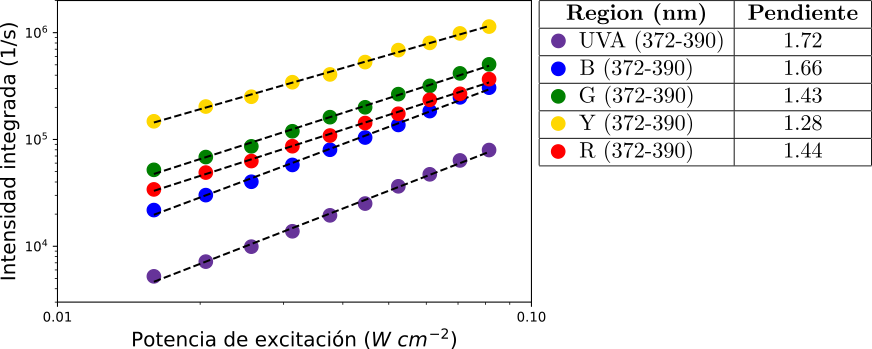
\includegraphics[width=\textwidth]{power_dep_ranges.png}
    \caption{\textbf{Gráfico Log-Log de I vs. P.} Codificado con colores se encuentran las intensidades para cada potencia de excitación para cada uno de las regiones del espectro definidas. La tabla muestra la pendiente de un ajuste lineal para cada rango.}
    \label{fig:power_dep_ranges}
\end{figure}

Como fue detallado en la sección \ref{sec:intro_ucnp}, la conversión ascendente es un proceso óptico no lineal en el que dos o más fotones se absorben secuencialmente entre niveles de energía igualmente espaciados, lo que lleva a la emisión de luz con una longitud de onda más corta que la incidente.  
Debido a las particularmente largas vidas medias (del orden de los cientos de microsegundos) y a los niveles de energía escalonados de los iones de tierras raras, se pueden observar espectros de conversión ascendente de UCNP en el rango visible incluso a bajas potencias de excitación.  
En este caso, medimos los espectros estáticos con densidades de potencia que varían entre 16 mW cm$^{-2}$ y 80 mW cm$^{-2}$ al excitar con el láser de forma continua (CW) (\textbf{Fig. \ref{fig:power_dep_spectrum}A}).  
El espectro estático muestra los picos de emisión conocidos de los iones Er$^{3+}$, que van desde la energía más baja hasta la más alta del espectro visible.  
Comenzando por el lado de menor energía, etiquetamos las regiones de emisión como rojo (R, 630–690 nm), amarillo (Y, 535–570 nm) y verde (G, 500–535 nm), correspondientes a las transiciones $^4$F$_{9/2} \to ^4$I$_{15/2}$, y $^4$S$_{3/2}, ^2$H$_{11/2} \to ^4$I$_{15/2}$, respectivamente.  
El espectro también muestra azul (B, 397–425 nm) y ultravioleta (UVA, 372–390 nm), que provienen de transiciones de niveles excitados más altos, como $^2$H$_{9/2} \to ^4$I$_{15/2}$ (410 nm) o $^4$G$_{11/2} \to ^4$I$_{15/2}$ (383 nm) \cite{haase_upconverting_2011}.  
Como se mencionó en la sección \ref{sec:intro_ucnp}, aunque las UCNPs muestran una relación no lineal entre la intensidad de emisión y la densidad de potencia de excitación, esto solo es apreciable cuando se abarcan varios órdenes de magnitud \cite{pollnau2000}.  
La intensidad de emisión de conversión ascendente ($I_{UC}$) está relacionada de manera no lineal con la densidad de potencia de excitación, $I_{UC} = P^\alpha$, donde $\alpha$ es el número efectivo de fotones involucrados en el proceso de absorción por fotón de mayor energía emitido, y $P$ es la potencia incidente \cite{Auzel2004}.  
El gráfico $\log{(I_{UC})}$ vs. $\log{(P)}$ (\textbf{Fig. \ref{fig:power_dep_ranges}}) muestra que, para este rango de potencias, cada región de emisión está caracterizada por una pendiente relacionada con el número de fotones involucrados en cada proceso (\textbf{Fig. \ref{fig:power_dep_ranges} inset}).  
No se observaron cambios en estas pendientes para cada longitud de onda (UV, B, G, R), lo que indica que los mecanismos fotofísicos que causan la conversión ascendente son los mismos para todas las potencias.  
Esto está en línea con el hecho de que la relajación cruzada y la transferencia de energía hacia atrás (BET) desde Er$^{3+}$ hacia Yb$^{3+}$ son despreciables en estos límites de baja potencia \cite{suyver_anomalous_2005} \cite{berry_disputed_2015}.


\begin{figure}[t]
    \centering
    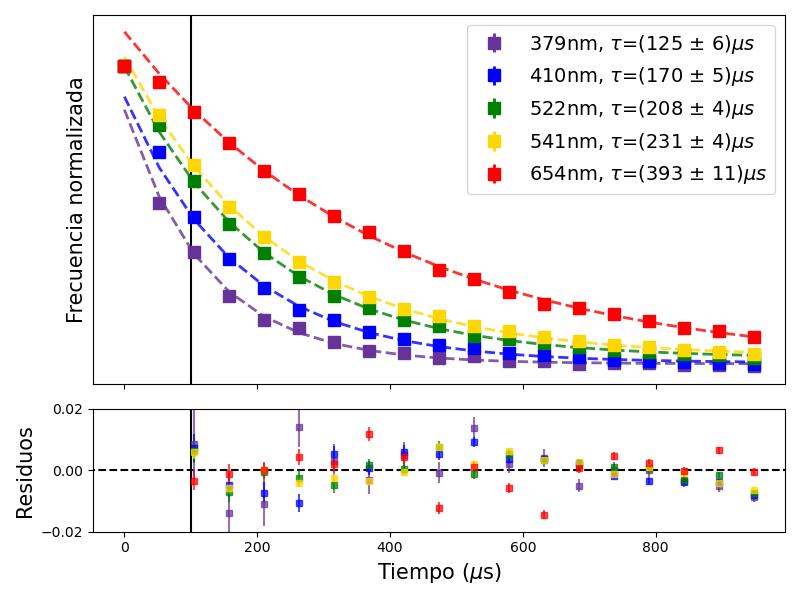
\includegraphics[width=\textwidth]{lifetimes_residuos.png}
    \caption{\textbf{Histogramas de tiempos de vida.} Tiempo de arribo de los fotones (cuadrados) y ajuste de decaimiento exponencial (líneas sólidas) para cada región del espectro. Los tiempos de vida se midieron a 976 nm, 0.087 mW cm$^{-2}$.}
    \label{fig:lifetimes}
\end{figure}

Además de obtener los espectros estacionarios de las UCNPs, medimos el tiempo de vida medio en los picos de emisión de cada una de las regiones espectrales (\textbf{Fig. \ref{fig:lifetimes}}), esto es para las longitudes de onda 379, 410, 522, 541 y 654 nm.
Ajustamos los histogramas de tiempo de arribo de los fotones con una curva de decaimiento monoexponencial, comenzando a los 100 $\mu$s después de que se detuvo la excitación para medir solo la desocupación de los estados excitados.  
El resultado son vidas medias que varían entre $\sim125$ y $\sim400$ $\mu$s.  
Se observa una disminución en la vida media para los fotones de longitud de onda más corta, correspondientes a estados excitados de mayor energía, lo que es consistente con un mayor número de vías de relajación. 
Por otro lado, se puede ver que los residuos no están uniformemente distribuidos.
Esto es esperable, ya que el modelo de decaimiento monoexponencial es un modelo efectivo para el comportamiento.
Como comentamos en la sección \ref{sec:intro_ucnp}, el modelo más completo para la dinámica de las UCNP consiste en 12 ecuaciones diferenciales ordinarias no lineales, con $\sim 50$ parámetros libres, en cambio nuestro modelo efectivo tiene un solo parámetro.
Adicionalmente, medimos el tiempo de vida para el pico de emisión de 541 nm a dos potencias distintas de excitación, 3 y 87 mW \textbf{\ref{fig:lifetimes_power}}.
Al igual que con la relación entre potencia e intensidad, el cambio en tiempo de vida no presenta diferencias significativas para el rango de potencias en el que medimos.

Para este rango de potencias de excitación, no se llegan a medir diferencias significativas ni en la relación funcinoal entre potencia e intensidad, ni en el tiempo de vida para el pico más intenso de emisión.
En el futuro, se podrían repetir las mediciones excitando a densidades de potencia en el rango de 10$^0$ mW cm$^{-2}$ y 10$^2$ mW cm$^{-2}$, en el que se observan cambios en la pendiente de los gráficos $\log(I)$ vs. $\log(P)$ \cite{bujjamer_luminescent_2020}.
Sin embargo, estas mediciones demuestran la posibilidad de realizar una caracterización óptica completa de las nanopartículas de \textit{upconversion} con las modificaciones que realizamos en el espectrofluorímetro QM 400.
Tanto las mediciones de espectro en función de la potencia como las de tiempo de vida fueron realizadas automáticamente con secuencias de comandos programadas en Python.
La plataforma permite desarrollar una secuencia de comandos más compleja que mida un espectro completo, detecte los picos de emisión y mida los tiempos de vida en esos picos, de forma que el usuario sólo tendría que colocar la muestra en la cámara y ejecutar el programa para realizar una caracterización óptica completa.




\begin{SCfigure}
    \centering
    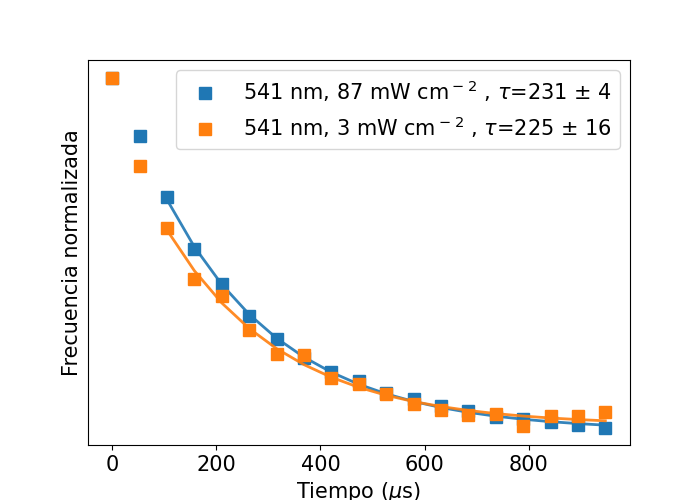
\includegraphics[width=0.7\textwidth]{lifetimes_power.png}
    \caption{\textbf{Tiempo de vida a distintas potencias.} Tiempo de arribo de los fotones (cuadrados) para el pico de emisión de 541 nm y dos potencias de excitación distintas, 3 mW cm$^{-2}$ y 87 mW cm$^{-2}$.}
    \label{fig:lifetimes_power}
\end{SCfigure}


\chapter{Conclusiones}
\renewcommand{\tablename}{\textbf{Tabla}}

Renovamos un espectrofluorímetro Horiba PTI Quanta Master 400 obsoleto.
Si bien sus elementos ópticos y de detección como los monocromadores y el PMT son componentes de altísima precisión, la utilización del instrumento resultaba dificultosa principalmente debido a su antigua PC de control con sistema operativo Windows 95.
Más allá de hacer tedioso su uso por la extracción de datos en disquette, la PC presenta una amenaza para la vida útil del fluorímetro: una falla en su funcionamiento puede dejarlo inutilizable y sin reparación, ya que el producto está fuera de soporte y sus partes no se consiguen en el mercado.
Nuestra renovación reemplazó la electrónica de control y la PC por una CPU y FPGA Red Pitaya, junto con dos paquetes de código abierto desarrollados en Python que cumplen el rol de \textit{software} de control y adquisición.
Para imitar el funcionamiento del fluorímetro original, hicimos una extensa caracterización del PMT y del algoritmo de conteo de fotones.

Además de la renovación, agregamos un láser externo pulsado de 980 nm que nos permitió adaptar el fluorímetro para hacer mediciones de espectros de emisión estáticos y dinámicos de nanopartículas de \textit{upconversion}.
Debido a los efectos no lineales que causan su luminiscencia, una caracterización óptica completa de estas partículas requiere medir sus espectros y tiempos de vida, del orden de milisegundos, para un rango de densidades de potencia de excitación.
Estas mediciones requieren el uso del fluorímetro por largos períodos de tiempo, en especial para potencias de excitación bajas en las que los tiempos de integración son largos.
Con nuestra plataforma estas mediciones se pueden programar en una rutina de Python, de forma tal que el usuario sólo debe depositar la muestra en la cubeta e iniciar la medición.

Por último, utilizamos nuestro desarrollo para hacer una caracterización óptica completa de UCNPs.
Las nanopartículas caracterizadas están compuestas por una matriz cristalina de fluoruro de ítrio dopada con iones lantánidos de iterbio y erbio, NaYF$_4$:Yb$^{+3}$,Er$^{+3}$, y fueron sintetizadas por el grupo de fotofísica del INQUIMAE, liderado por Beatriz Barja y María Claudia Marchi. 
Medimos su espectro estacionario y tiempos de vida para los picos de emisión en un rango de densidades de potencia entre 16 mW cm$^-1$ y 80 mW cm$^-1$.
Si bien los mecanismos no lineales de interacción entre los dopantes de las nanopartículas hacen que éstas tengan una respuesta no lineal con la potencia, no vemos ese comportamiento en nuestras mediciones.
Esto es porque el rango de potencias en el que excitamos es demasiado pequeño como para que haya un cambio en los mecanismos de \textit{upconversion}.

De cara al futuro, vemos que hay tres líneas en las que se puede progresar: (i) realizar mejoras en la plataforma que ya desarrollamos, (ii) aplicar nuestra plataforma a otros fluorímetros y (iii) aprovechar la automatización del instrumento para hacer mediciones más inteligentes.
En primer lugar, si bien la plataforma que desarrollamos cumple con la tarea de poder caracterizar UCNPs y renovar el fluorímetro, muchas de sus partes, como la GUI y la placa con la conexión a los instrumentos no son robustas.
Ahora que demostramos que las modificaciones funcionan, se podrían diseñar placas PCB, comprar conectores estandar y mejorar la GUI.

En segundo lugar, una vez que tengamos un diseño más robusto de las partes podríamos aprovechar para aplicar la renovación a los fluorímetros presentes en los institutos de Buenos Aires.

Por último, como se comentó en la introducción, la interacción entre los dopantes de las UCNPs se puede modelar con un sistema de ODEs con $\sim 50$ parámetros desconocidos.
Ajustar este modelo haciendo mediciones variando la potencia de excitación, longitud de onda de medición y ciclo de trabajo con fuerza bruta resulta impráctico.
En cambio, con nuestra plataforma se podría implementar un algoritmo que tome mediciones, haga un ajuste en tiempo real, y determine cuál es la próxima medición más informativa a realizar.
De esa forma, nuestra plataforma nos permitiría estudiar los mecanismos internos de interacción de las nanopartículas de \textit{upconversion}. 





\bibliography{citas}
\bibliographystyle{rsc}

\begin{appendices}

\renewcommand{\thesection}{\Alph{section}}
\renewcommand{\thefigure}{A\arabic{figure}}
\renewcommand{\tablename}{Tabla}
\renewcommand{\thetable}{A\arabic{table}}

\section{instrucciones de armado} \label{apendice:instrucciones_armado}

\subsection{Renovación del Horiba PTI Quanta Master 400} \label{subsec:refur-instructions}

El proceso de ensamblaje para la renovación del espectrómetro Horiba PTI Quanta Master 400 se puede organizar en cinco pasos: (1) conectar el motor de excitación $M_1$ (\textbf{Fig. \ref{fig:hardware}}), (2) conectar el fin de carrera de excitación, (3) conectar el motor de emisión $M_2$, (4) conectar el fin de carrera de excitación y (5) conectar la salida del PMT. 
Las fuentes de alimentación deben permanecer apagadas hasta que todo esté correctamente conectado, como se muestra en el esquema (\textbf{Fig. \ref{fig:schematic}}). 
Es necesario asegurarse de que el voltaje de GND sea el mismo en todas las conexiones. 
\textbf{Advertencia:} configurar límite de corriente del controlador DRV8825 esté configurado correctamente (en nuestro caso, para limitar a 0.7 A) y que los pines estén conectados adecuadamente, de lo contrario existe el riesgo de que circule demasiada corriente por los bobinados de los motores y se dañen.

\begin{enumerate}
    \item \textbf{Conectar el motor de excitación}
    \begin{enumerate}
        \item Conectar los pines P6 y P7 del RP a los pines STEP y DIR del DRV8825, respectivamente (\textbf{Fig. \ref{fig:schematic}}).
        \item Conectar los pines restantes: utilizando 3.3 V del RP como nivel alto digital, coloque los pines $\overline{\text{SLEEP}}$ y $\overline{\text{RESET}}$ del controlador del motor en alto, y conecte el GND lógico al GND del RP. Los pines $\overline{\text{ENABLE}}$, M0, M1, M2 y $\overline{\text{FAULT}}$ pueden dejarse flotantes.
        \item Ajustar el límite de corriente de salida del DRV8825 al máximo soportado por el motor paso a paso; en este caso, el motor M061CS02 tiene un límite de 0.7 A.
        \item Provea la fuente de alimentación del motor conectando los pines VMOT y GND a una fuente de 12 V que pueda suministrar al menos $2 \times \textit{límite de corriente}$. Conectar un capacitor de 100 $\mu F$ en paralelo.
        \item Conectar el controlador del motor al motor paso a paso: desconecte el conector original del motor $M_1$ y conecte los pines A1 y A2 del DRV8825 a los pines 1 y 7 del motor, y los pines B1 y B2 a los pines 3 y 5 (\textbf{Fig. \ref{fig:hardware}B}).
    \end{enumerate}
    \item \textbf{Conectar el fin de carrera de excitación}
    \begin{enumerate}
        \item Alimentar con 5 V y GND a los pines 1 y 2, respectivamente, del fin de carrera junto al motor $M_1$ (\textbf{Fig. \ref{fig:hardware}C}).
        \item Conectar el pin 3 del fin de carrera al pin digital P2 del RP para el fin de carrera de $M_1$, utilizando una resistencia pull-up externa al nivel lógico de 3.3 V del RP.
    \end{enumerate}
    \item \textbf{Conectar el motor de emisión}
    \begin{enumerate}
        \item Conectar los pines P4 y P5 del RP a los pines STEP y DIR del controlador del motor, respectivamente.
        \item Repetir los pasos (b) a (e) del ítem (1) para el motor $M_2$.
    \end{enumerate}
    \item \textbf{Conectar el fin de carrera de emisión}
    \begin{enumerate}
        \item Alimentar con 5 V y GND a los pines 1 y 2, respectivamente, del fin de carrera junto al motor $M_2$ (\textbf{Fig. \ref{fig:hardware}C}).
        \item Conectar el pin 3 del fin de carrera al pin digital P3 del RP para el fin de carrera de $M_2$, utilizando una resistencia pull-up externa al nivel lógico de 3.3 V del RP.
    \end{enumerate}
    \item \textbf{Conectar la salida del PMT}
    \begin{enumerate}
        \item Conectar el cable BNC-SMA a la entrada analógica 1 del RP y configure el modo de alto voltaje.
        \item Conectar una ficha T BNC al extremo BNC del cable BNC-SMA conectado al RP.
        \item Conectar una terminación de 50 $\Omega$ a uno de los extremos de la ficha T para conformar pulsos de 40 a 100 ns.
        \item Conectar el otro extremo de la ficha T a la salida del PMT utilizando un cable BNC-BNC.
    \end{enumerate}
\end{enumerate}

\noindent Después de estos pasos, el instrumento estará listo para realizar mediciones estacionarias.

\begin{SCfigure}[][h]
         \centering
         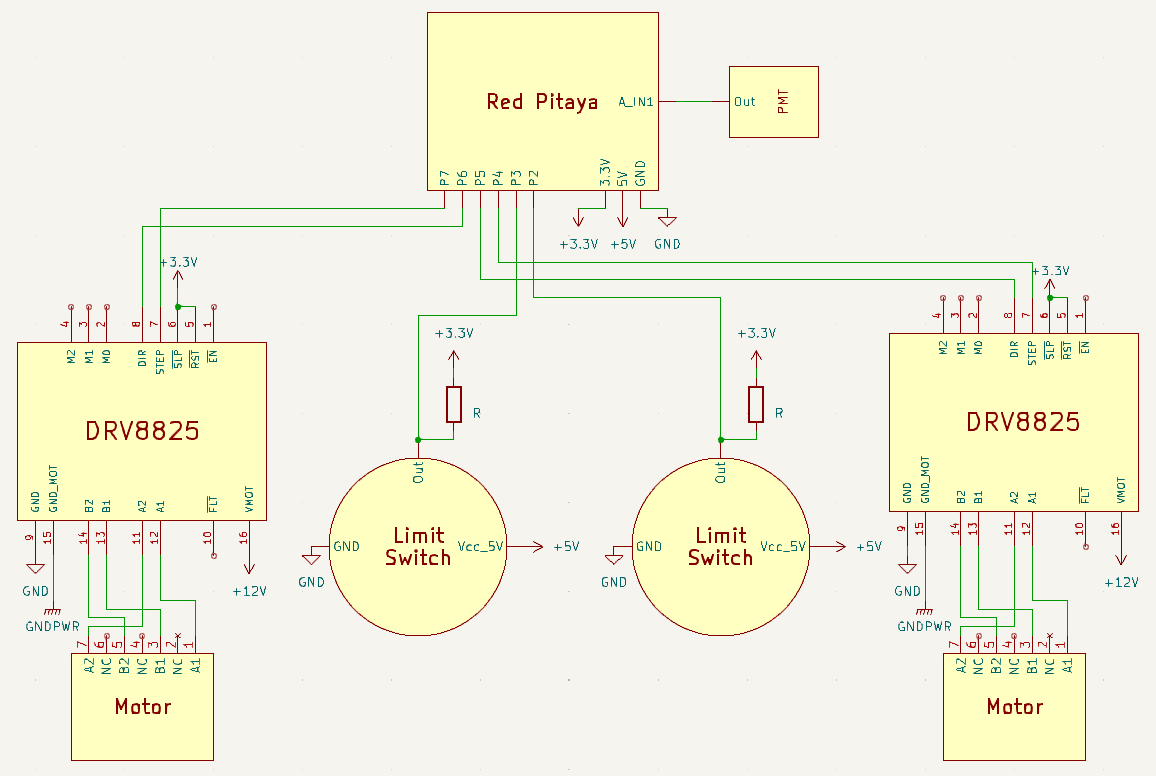
\includegraphics[width=.65\textwidth]{schematic.png}
         \caption{\textbf{Esquemático de las conexiones} que contiene la placa PCB de prueba para conectar las componentes del hardware a la RP.
         }
         \label{fig:schematic}
    \end{SCfigure}


\subsection{Ampliación para mediciones dinámicas}

Para añadir la funcionalidad de medir tiempos de vida con el espectrómetro Horiba PTI, además de las instrucciones anteriores, deben realizarse los siguientes pasos adicionales:

\begin{enumerate}
    \item Conectar la fuente de luz externa al puerto externo utilizando un cable de fibra óptica.
    \item Conectar el puerto USB tipo B del ITC4020 al puerto USB tipo A del RP.
    \item Conectar la salida BNC R3 (salida TTL de 5 V del ITC4020) en el panel trasero del ITC4020 a un adaptador BNC a SMA, y luego conectarlo a la entrada analógica 2 del RP configurando ese canal en modo de alto voltaje.
\end{enumerate}

Nuestro software está diseñado para trabajar con el controlador láser ITC4020, pero se puede utilizar otro siempre y cuando se añadan clases de control específicas al software.

\subsection{Instalación y configuración del software} 

Seguir las instrucciones en \href{https://github.com/tdinapoli/refurbishedPTI}{este enlace}\cite{napoli_tdinapoli_2024} para instalar nuestro paquete Python en su RP. 
Una vez conectados los componentes de hardware, se deben calibrar los motores de los monocromadores y las entradas analógicas del Red Pitaya. 
Las instrucciones para calibrar las entradas analógicas del RP están disponibles en su documentación oficial \cite{rp_docs}.

Para calibrar los monocromadores, desarrollamos un intérprete de línea de comandos que guía el proceso paso a paso y genera un archivo YAML con los parámetros de calibración (\textbf{Tabla \ref{tab:monochromator_api_parameters}}). El siguiente código en Python abre el menú para calibrar el monocromador de emisión:

\begin{lstlisting}[language=Python]
from refurbishedPTI import Spectrometer
spec = Spectrometer.constructor_default()
spec.emission_mono.calibrate()
\end{lstlisting}

El comando \texttt{save\_to\_yaml} guarda el archivo de configuración en el directorio del RP indicado por el método \texttt{.get\_config\_path()} de la clase Motor. Una vez calibrado el monocromador de emisión, repita el proceso para el monocromador de excitación:

\begin{lstlisting}[language=Python]
spec.excitation_mono.calibrate()
\end{lstlisting}

Repetir los mismos pasos que para el monocromador de emisión para completar la configuración.

\begin{table}[h]
 \centering
 \begin{tabular}{|l|l|p{10cm}|}
    \hline
    \textbf{Parámetro} & \textbf{Tipo de dato} & \textbf{Descripción} \\ \hline
    \texttt{greater\_wl\_cw}          & bool               & True si la longitud de onda incrementa al girar en sentido horario, Falso en el caso contrario. \\ \hline
    \texttt{max\_wl}                 & float              & Longitud de onda máxima (en nanómetros) que permitirá configurar la API del monocromador \\ \hline
    \texttt{min\_wl}                 & float              & Longitud de onda mínima (en nanómetros) que permitirá configurar la API del monocromador \\ \hline
    \texttt{wl\_step\_ratio}          & float              & Cambio (en nanómetros) de longitud de onda por cada paso que da el motor.\\ \hline
    \texttt{home\_wavelength}        & float              & Longitud de onda (en nanómetros) en la que se activa la señal del fin de carrera. \\ \hline
\end{tabular}
\caption{\textbf{Parámetros de la API de la clase Monochromator.}}
\label{tab:monochromator_api_parameters}
\end{table}

\section{Instrucciones de uso} \label{apendice:instrucciones_uso}

Como se comentó en la sección \ref{sec:software}, hay dos formas de operar el espectrómetro renovado: a través de la API de Python y mediante la interfaz gráfica Jupyter Notebook con IPython Widgets. 

Para ambos modos de operación, todos los instrumentos listados en la explicación de la sección \ref{subsec:refur-instructions} deben estar conectados, y tanto el PMT como la lámpara deben estar encendidos. 
Se deben ajustar las rendijas de Em y Ex (\textbf{Fig. \ref{fig:ref-diagram}}) según las necesidades del experimento. 
Una vez completados estos pasos, se puede proceder con las siguientes secciones para el modo de operación por script o GUI.

\subsection{Modo de operación GUI}

La interfaz gráfica del espectrómetro se encuentra en un Jupyter Notebook que permite al usuario cambiar los parámetros del instrumento mediante Widgets de Jupyter.  
La GUI se compone de dos secciones: el panel de parámetros y el panel de gráficos (\textbf{Figs. \ref{fig:spectrum_gui}} y \textbf{\ref{fig:lifetime_gui}}).  
El panel de parámetros contiene menús desplegables, botones y campos de texto para especificar los parámetros de medición y del archivo de medición.  
El panel de gráficos incluye dos gráficos, uno para mediciones de espectro y otro para mediciones de tiempo de vida.  

Para inicializar el modo GUI del QM400 renovado, se debe abrir el notebook \texttt{gui.ipynb} ubicado en \texttt{/home/jupyter/refurbishedPTI/gui.ipynb}.  
Al ejecutar la primera celda del notebook con el código:

\begin{lstlisting}[language=Python]
from refurbishedPTI.gui import Gui
gui = Gui()
\end{lstlisting}

\noindent se inicializa la GUI. 

Para realizar una medición seleccionar las opciones \textbf{Spectrum} o \textbf{Lifetime} en el menú desplegable \textbf{Measurement type}.  
Se especifican los parámetros de la medición utilizando los componentes de la GUI (detallados en las \textbf{Tablas \ref{tab:spectrum_measurement}} y \textbf{\ref{tab:lifetime_measurement}}) y comenzar la adquisición.  
Una vez finalizada la medición, guarde y manipule los datos con los componentes de la GUI (\textbf{Tabla \ref{tab:file_parameters}}).

\begin{table}
    \centering
    \begin{tabularx}{\textwidth}{|l|X|}
        \hline
        \textbf{Parameter Name} & \textbf{Description} \\
        \hline
        \multirow{3}{3cm}{Spectrum type} & \textbf{Emission}: fixed excitation monochromator and scanning emission monochromator. \\
        \cline{2-2}
        & \textbf{Excitation}: fixed emission monochromator and scanning excitation monochromator. \\
        \cline{2-2}
        & \textbf{Laser}: scanning emission monochromator external laser excitation. \\
        \hline
        Static monochromator wavelength & Fixed monochromator wavelength (nm). \\
        \hline
        Starting wavelength & Starting wavelength of the scanned wavelength range (nm). \\
        \hline
        Ending wavelength & Ending wavelength of the scanned wavelength range (nm). \\
        \hline
        Wavelength step & Difference in wavelength between each data point (nm). \\
        \hline
        Acquire & Starts the measurement. \\
        \hline
    \end{tabularx}
    \caption{\textbf{Parámetros de configuración de una medición de espectro estático}.}
    \label{tab:spectrum_measurement}
\end{table}

\begin{table}[htbp]
    \centering
    \begin{tabularx}{\textwidth}{|l|X|}
        \hline
        \textbf{Parameter Name} & \textbf{Description} \\
        \hline
        Pump power & Laser pump power (mW). \\
        \hline
        Frequency & Laser on and off TTL signal frequency. \\
        \hline
        Duty Cycle & Duty cycle of TTL signal in \%. \\
        \hline
        Emission monochromator wavelength & Wavelength at which the lifetime will be measured (nm). \\
        \hline 
        Amount of counts & Amount of counts that will be measured until the measurement ends. \\
        \hline
        Starting time & Time after trigger before start counting (ms). \\
        \hline
        Ending time & Time after trigger before stop counting (ms). \\
        \hline
        Acquire & Starts the measurement.\\
        \hline
    \end{tabularx}
    \caption{\textbf{Parámetros de configuración de una medición dinámica}.}
    \label{tab:lifetime_measurement}
\end{table}

\begin{table}[htbp]
    \centering
    \begin{tabularx}{\textwidth}{|l|X|}
        \hline
        \textbf{Parameter Name} & \textbf{Description} \\
        \hline
        Measurement filename & Select a filename and directory where the measurement will be saved once the \textbf{Save} button is pressed. If no filename is selected at the time of pressing the \textbf{Acquire} button, the filename will be the current date and time. \\
        \hline
        Selected measurement & Select a measurement to \textbf{Save} it or \textbf{Delete} it. \\
        \hline
        Save & Save measurement with selected filename, directory, and format. \\
        \hline
        Delete & Delete selected measurement. \\
        \hline
        \multirow{3}{3cm}{Save to} & File format for the saved measurement. Options: \\
        \cline{2-2}
        & \textbf{pickle} \\
        \cline{2-2}
        & \textbf{csv} \\
        \cline{2-2}
        & \textbf{excel} \\
        \hline
    \end{tabularx}
    \caption{\textbf{Parámetros de configuración del archivo que guarda los datos de una medición}.}
    \label{tab:file_parameters}
\end{table}

\begin{figure}
    \centering
    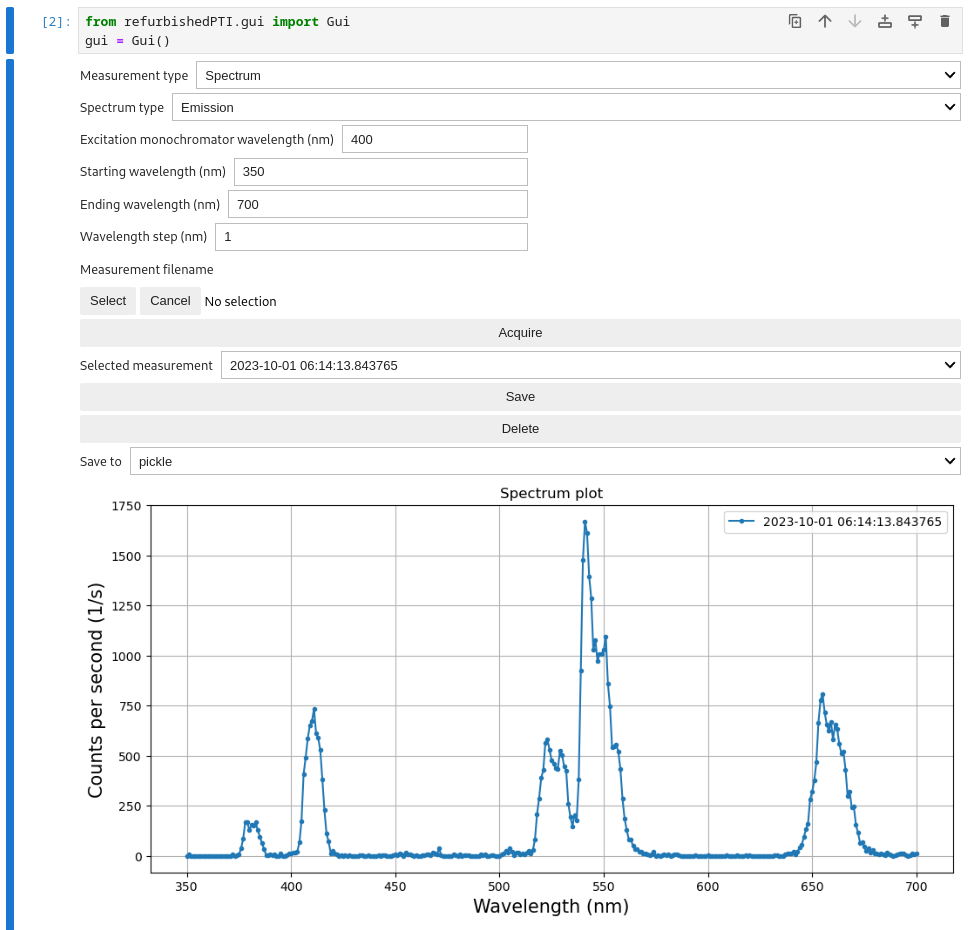
\includegraphics[width=\textwidth]{spectrum_gui.png}
    \caption{\textbf{GUI para medir espectros estacionarios}.}
    \label{fig:spectrum_gui}
\end{figure}

\begin{figure}
    \centering
    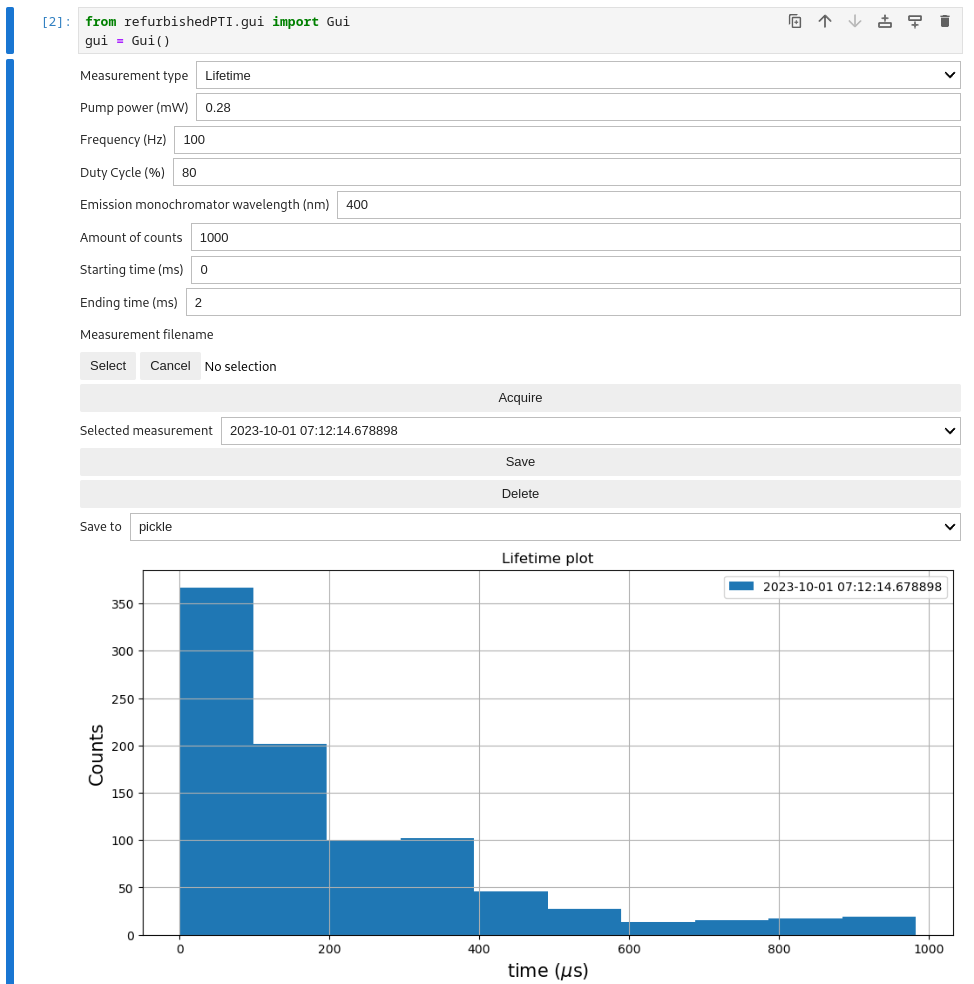
\includegraphics[width=\textwidth]{lifetime_gui.png}
    \caption{\textbf{GUI para medir tiempos de vdia}.}
    \label{fig:lifetime_gui}
\end{figure}


\section{tiempos de vida todos los picos a != pot}
\section{analisis picos}
\section{benchmark}
\end{appendices}

\end{document}

